%!TEX root = ../thesis.tex
%*******************************************************************************
%****************************** Third Chapter **********************************
%*******************************************************************************
\chapter{Discrete model} \label{ch:3}

% **************************** Define Graphics Path **************************
\ifpdf
    \graphicspath{{Chapter3/Figs/Raster/}{Chapter3/Figs/PDF/}{Chapter3/Figs/}}
\else
    \graphicspath{{Chapter3/Figs/Vector/}{Chapter3/Figs/}}
\fi

Models of organisms and population dynamics must be designed by either describing potentially many discrete units\footnote{in this case, cells} with continuous functions or dealing with the analytical complexity of discretisation. 
Even with the continuous description of \textit{C. flexa} described previously, numerical solutions to the shape equations would require discretisation of a surface. 
Here, I pursue a simplified, discrete description of \textit{C. flexa} sheets. 
As in \cref{ch:2}, I proceed by formulating an energy function based on the coordinate vectors of cells and vary it with respect to the coordinates. 
This procedure results in expressions for the forces on the coordinates, which can be forward integrated in time to study the dynamics and steady state geometries of \textit{C. flexa} sheets.

In addition to avoiding the complexity of describing surface curvatures $H, K$ in a discrete program, the discrete approach gives force equations that are relatively quite tractable. 
Expressing the gradient of the energy as summations over collars belonging to each cell or cell-cell interactions makes it possible to neatly arrange the force calculations as tensor index contractions or, even more simply, matrix multiplications. 
The dynamics can efficiently be solved numerically as a result.
Of course, describing choanoflagellate sheets as discrete systems also remains faithful to real sheets, and this approach remains applicable over colonies of arbitrarily many cells.

In \cref{sec:description}, I discuss the reasoning behind the discrete model that I choose to use: why cells and collar boundary endpoints are used as the vertices, how the apicobasal axis unit vector is determined, why collar-collar connections at the sheet boundary matter, and how initial sheet geometries are set up numerically.
The following \cref{sec:sheet_energy} proceeds to write an equation for the mechanical energy of the sheet in terms of cell positions and cell-cell interface endpoint coordinates, as well as the apicobasal axis unit vectors as free variables.
\Cref{subsec:grad_desc}-\ref{subsec:forward_int} proceed to minimise energy by following the negative gradient\footnote{Equivalently, equilibrate forces.}, and the remainder of \cref{sec:minimise_energy} discusses the solutions observed under various sheet graph topologies.


\section{Discrete sheet description} \label{sec:description}

\nomenclature[a-G]{$G$}{Graph consisting of \textit{C. flexa} cells as vertices and cell-cell interactions through collar microvilli as edges}
\nomenclature[a-Gs]{$G^*$}{Graph consisting of collar microvillar interfaces between cells as edges and interface endpoints as vertices}
\nomenclature[g-ps]{$\rho,\sigma$}{Indices used to index collar vertices in the discrete sheet description $\mathfrak{G}$}
\nomenclature[g-ab]{$\alpha,\beta$}{Indices used to index cell vertices in the discrete sheet description $\mathfrak{G}$}
\nomenclature[g-g]{$\gamma$}{Index for either cell ($\alpha,\beta$) or collar ($\rho,\sigma$) vertices in the discrete sheet description $\mathfrak{G}$}
\nomenclature[s-ap]{$(\alpha,\rho)$}{Index for cell $\alpha$ and collar vertex $\rho\subset\alpha$. The set of cell, collar pairs is treated as ordered}
\nomenclature[s-abps]{$(\alpha,\beta:\rho,\sigma)$}{Index for the interface given by collar vertices $\rho,\sigma$ for cells $\alpha,\beta$. The set of these indices is treated as ordered}
\nomenclature[a-n]{$\bh{n}_\alpha$}{Cell body orientation vector for cell $\alpha$. Unit vector}
\nomenclature[a-rvec]{$\bm{r}_\gamma$}{Vector position of vertex $\gamma$}
\nomenclature[x-apvec]{$\vec{\alpha\rho}$}{Vector between vertices $\alpha$ and $\rho$, $\bm{r}_\rho - \bm{r}_\alpha$}
\nomenclature[g-ph]{$\phi$}{Denotes the angle between a cell orientation vector and cell-to-collar vector (\cref{eq:phi}). Indexed $\phi_{(\alpha, \rho)}$ for cell $\alpha$, collar $\rho$}
\nomenclature[g-ps]{$\psi$}{Denotes half the angle between two collar interfaces (\cref{eq:psi}). Indexed $\psi_{(\alpha,\beta:\rho,\sigma)}$ for cells $\alpha,\beta$ and mutual collar endpoints $\rho,\sigma$}
\nomenclature[x-e]{$\e$}{Total sheet energy. In the discrete sheet description, $\e = \e_\phi+ \e_\psi+ \e_{\text{sp}}$ is the sum of energies for angles $\phi$ and $\psi$ and collar length, respectively. An adjustment $\e_\varphi$ is later added for numerical stability.}

The most natural framework to describe a set of interactions between discrete points is graph theory. 
Since colonies of \textit{C. flexa} form sheets with two distinct sides and there is no evidence to suggest that \textit{Choanoeca} acts otherwise \citep{brunet2019,leadbeater1983}, we are welcome to treat the network of interactions between cells as a plane graph $G$. 
With cells $C = \{\alpha\}_{\alpha\in C}$ making up vertices and cell-cell interactions via collars $E = \{(\alpha, \beta)\}_{(\alpha,\beta)\in E}$ making up edges in a graph $G$, we describe which cells impart forces on each other.

However, we understand from the studies into \textit{Choanoeca} that cells interact through their collars \citep{ellis1930,leadbeater1983,brunet2019}. 
Guided by imaging in the sheet-tangential plane (\cref{subfig:contact1,subfig:contact2}), we see that another natural planar graph $G^*$ is that with edges along interfaces between cells' collars.\footnote{Until noted otherwise, I treat the several collars interacting between two cells as a continuous line of interaction with infinitesimal collars spanning the cells' interface. The implications of this choice are discussed later.} 
In this description, vertices mark the points at which the interface between a pair of cells $(\alpha, \beta)\in E$ ends. 
For a cell $\alpha\in C$ whose collar microvilli are all in contact with those of other cells, the vertices in $G^*$ corresponding to cell $\alpha$ are points where $\alpha$ interacts with two or more cells simultaneously.

\begin{figure}[htbp]
    \centering
    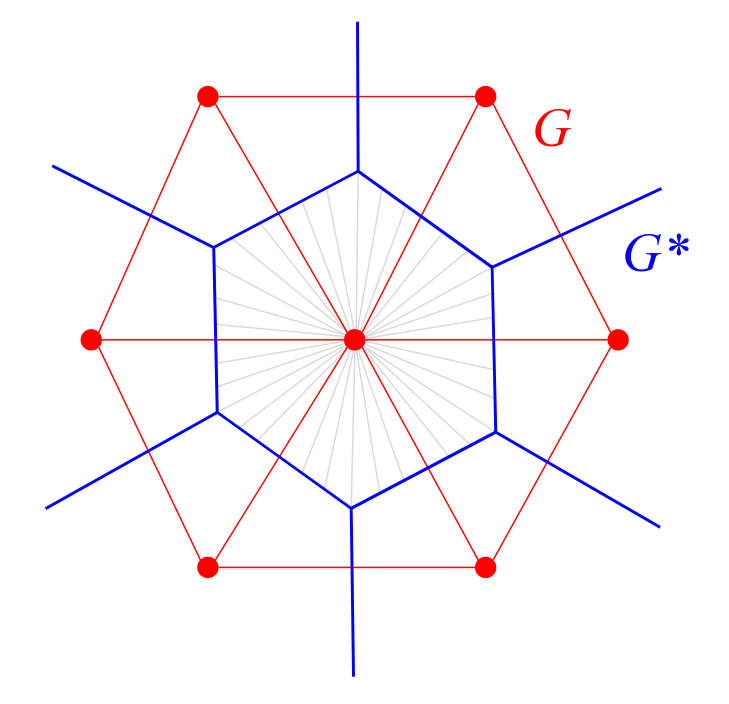
\includegraphics[width=0.6\textwidth]{duals.png}
    \caption[Planar dual graphs describing \textit{C. flexa} colonies]{Planar dual graphs describing \textit{C. flexa} colonies. The graph of cells and cell-cell interactions $G$ shown in red and collar interfaces $G^*$ shown in blue. Compare to \cref{subfig:contact1}, with prominent cell bodies and lines of interface between neighbouring cells' collars.}
    \label{fig:duals}
\end{figure}

As each edge in $G^*$ transects an edge $(\alpha, \beta)$ between cells $\alpha, \beta$ in $G$, we identify $G^*$ as the dual graph of $G$ (\cref{fig:duals}). \footnote{As $G$ is finite, all vertices in $G^*$ as described above which indicate two cells' interactions ending at the edge of a colony sheet would be merged into a single vertex $v_*$ in the dual graph of $G$. Consequently $G^*$ is not exactly the dual graph of $G$. We address this later when defining sheet edges numerically by replacing each edge $(v, v_*)$ in $G^*$ with the edge $(v, v')$ for new vertices $v'$ and removing $v_*$ from $G^*$ and deleting all edges incident on $v_*$.}
Consequently, we have that either $G$ or $G^*$ is sufficient to specify the topology of the other provided the coordinates of vertices. 

For the remainder of this chapter, I will use indices $\alpha,\beta$ to index cell vertices in $G$, indices $\rho, \sigma$ to index collar-collar interface boundary vertices in $G^*$, and index $\gamma$ to index either type of vertex.

\subsection{Defining a sheet} \label{subsec:springs}

A reasonable simplification of the cell sheet will use either the cell-cell interaction graph $G$ or the collar boundary edge graph $G^*$. 
Since physical interactions occur at the collar interfaces, I consider first the physical details of a model defined on $G^*$. 
The following analysis establishes that it is reasonable to consider only the endpoints of lines along which cells' collars interact, at the meeting points of blue lines in \cref{fig:duals}.

If two cells have a collar boundary described by $\bm{r}_\rho t + (1-t)\bm{r}_\sigma$ with $0 \leq t \leq 1$ and the energy is defined by continuously many springs from the boundary to a projected cell point $\bm{r}^*_\alpha$, then the energy $E_{\rho\sigma}$ of that boundary is 
 \begin{align}
     E_{\rho\sigma} = \int_0^1 \left[(\bm{r}_\rho t + (1-t)\bm{r}_\sigma) - \bm{r}^*_\alpha \right]^2 dt &= \frac{1}{3} (\bm{r}_\rho + \bm{r}_\sigma)^2 - \frac{1}{3} \bm{r}_\rho\cdot\bm{r}_\sigma - \bm{r}^*_\alpha \cdot (\bm{r}_\sigma + \bm{r}_\sigma) + \bm{r}^{*2}_\alpha. \label{eq:eab}
 \end{align}

The energy corresponding to a cell consists of the line energies of all the collar interfaces. 
We find the position $\bm{r}^*_\alpha$ by setting the gradient of equation \ref{eq:eab} with respect to $\bm{r}^*_\alpha$ to zero for all lines $\rho\sigma$. 
If $\rho$ indexes the vertices that cell $\alpha$ has (which I denote $\rho\subset\alpha$ for the remainder of this chapter), then 
\begin{align*}
    0 = \frac{dE}{d\bm{r}^*_\alpha} &= -\sum_{\rho\subset\alpha} \bm{r}_\sigma + 2d_\alpha\bm{r}^*_\alpha \\
    \bm{r}^*_\alpha &= \frac{1}{d_\alpha} \sum_{\rho\subset\alpha} \bm{r}_\rho
\end{align*}
\noindent for total stretching energy $E = \sum_{\rho\sigma}E_{\rho\sigma}$ and number of collars $d_\alpha$ belonging to $\alpha$.

The force on vertex $\sigma$ is then given by the negative gradient of the whole sheet energy $E$, which is the sum of the energies corresponding to each cell $\alpha$: 
\begin{align*}
    \frac{d E}{d\bm{r}_\sigma} &= \frac{d}{d\bm{r}_\sigma} = \sum_{\alpha:\sigma \subset \alpha} \frac{d}{d\bm{r}_\sigma} \sum_{\rho \subset \alpha} (\bm{r}_\rho - \bm{r}^*_\alpha)^2. 
\end{align*}
\noindent Since $\bm{r}_\alpha^*$ depends on $\bm{r}_\rho$ itself, we write
\begin{align}
	-\frac{dE}{d\bm{r}_\sigma} &= \sum_{\alpha:\sigma \subset \alpha} \frac{d}{d\bm{r}_\sigma} \sum_{\rho \subset \alpha} \left(\bm{r}_\rho - \frac{1}{d_\alpha} \sum_{\gamma\subset\alpha}\bm{r}_\gamma\right)^2 \nonumber \\
	&= \sum_{\alpha:\sigma\subset\alpha} \sum_{\rho\subset\alpha}\left( 2\bm{r}_\sigma \delta_{\sigma\rho} -\frac{2}{d_\alpha} \sum_{\gamma\subset\alpha}(\bm{r}_\gamma \delta_{\sigma\rho} + \bm{r}_\rho \delta_{\sigma\gamma}) + \frac{1}{d_\alpha^2} \sum_{\upsilon\subset\alpha}\sum_{\nu\subset\alpha} (\bm{r}_\nu \delta_{\sigma\upsilon} + \bm{r}_\upsilon \delta_{\sigma\nu}) \right) \nonumber \\
	&= -2 \sum_{\alpha: \sigma\subset\alpha} (\bm{r}_\sigma - \bm{r}_\alpha^*). \label{eq:com}
\end{align}

\Cref{eq:com} aligns with the expectation that the forces on $\bm{r}_\sigma$ are linear based on the difference to the projected cell points $\bm{r}_\alpha^*$ that $\sigma$ belongs to, owing to the linearity of the entire system.
While the answer may have been readily guessed, the above process of solving for the forces on $\bm{r}_\sigma$ are necessary for nonzero collar length $\ell_0$. 

If instead the line energy is 
\begin{align*}
    E_{\rho\sigma} &= \int_0^1 \left(\left|\bm{r}_\rho t + (1-t)\bm{r}_\sigma - \bm{r}_\alpha^*\right| - \ell_0 \right)^2 dt,
\end{align*}
then the cell position $\bm{r}^*_\alpha$ is the solution to
\begin{align}
	0 &= -2\sum_{\rho\subset\alpha} \bm{r}_\rho + 2d_\alpha \bm{r}_\alpha^* -2\ell_0 \frac{d}{d\bm{r}_\alpha^*} \sum_{(\rho,\sigma) \text{ edge of }\alpha} \int_0^1 \frac{\bm{r}_\alpha^* - \bm{r}_\sigma - t (\bm{r}_\rho - \bm{r}_\sigma)}{| \bm{r}_\rho t - (1-t) \bm{r}_\sigma - \bm{r}_\alpha^*|} dt \label{eq:com_full}
\end{align}

Although the integral in \cref{eq:com_full} can be evaluated analytically, it results in a transcendental equation for $\bm{r}_\alpha^*$. 
Despite the complexity of nonzero equilibrium length for finding a cell position, I nevertheless use the result that continuous spring interfaces can be effectively distilled to interface endpoints (\cref{eq:com}) in the model developed in \cref{subsec:init}.

\subsubsection{Bending} \label{subsubsec:bending}

Points corresponding to cell bodies and collar-collar interface edges make it simple to describe a physically realistic bending energy, though it is not as clear how to define a bending energy.

\citet{seung1988} describe triangulated surfaces and define a bending energy between two triangles $\alpha,\beta$ sharing an interface $\rho, \sigma$ as contributing bending energy $|\bh{n}_\alpha - \bh{n}_\beta|^2/2 = 1 - \bh{n}_\alpha \cdot \bh{n}_\beta$, where all normals face on the same side of the surface. 
Indeed, the continuous approximation of this energy function for small difference $\bh{n}_\alpha - \bh{n}_\beta$ gives the Helfrich energy density $4H^2 - 2K$ \citep{helfrich1973}. 
When cells make boundaries with more than three cells simultaneously, there is not an immediately clear way to define the normal vector $\bh{n}_\alpha$ of a cell $\alpha$. 

As I discuss later (\cref{subsubsec:approx_norm}), a reasonable choice that does not depend on cell position (which in this case is already projected onto the approximated plane of collar positions) would be to approximate $\bh{n}_\alpha$ as the normal vector of a plane approximation to the collar vectices $\bm{r}_\rho$ for $\rho\subset\alpha$. 
Although this choice is intuitively reasonable, it lacks physical motivation as it does not necessarily minimise the energy when the cell body is considered (\cref{subsubsec:opt_norm}).
On the other hand, treating the normal vectors as free variables here would allow them to take any direction to minimise the energy, which does not translate to any physical movement or rotation of the cell body. 

\subsection{Surface formed by cell bodies}

The other natural, minimal discrete description of \textit{C. flexa} is to include only cell coordinates and the network of cell-cell interactions (\cref{sec:description}).
Again, we look to describe the energy contributed by collar stretching and sheet bending.
Unlike the description of bending in \cref{subsubsec:bending}, knowledge of cell body positions gives cell orientation vectors $\bh{n}_\alpha$ a clear physical significance.
Defining the $\bh{n}_\alpha$ as free vectors removes any ambiguity and a bending energy $1 - \bh{n}_\alpha \cdot \bh{n}_\beta$ for two cells $\alpha, \beta$ is reasonable.

On the other hand, considering only cell positions gives no clear method for defining a stretching energy based in a physical mechanism.
We may proceed to define both bending and stretching energy by solving for the minimum energy curves describing two filaments meeting at some mutual point and tangent angle as functions of cell body orientation vectors $\bh{n}_\alpha, \bh{n}_\beta$ and vector $\bm{r}_\alpha - \bm{r}_\beta$ between the two cells.
For any description of cell-cell interactions in \textit{C. flexa} sheet, this approach by treating each collar as a linear filament would likely be the most accurate as it does not require any simplification into angles $\phi, \psi$ (\cref{eq:phi,eq:psi}).
However, this level of complexity removes the interpretational and computational simplicity of distilling the problem as I sought. 
Since neither approach here nor in \cref{subsec:springs} captures all physical interactions in a \textit{C. flexa} sheet with clearly defined terms, I decided to pursue an approach that used details of both collar interactions and cell positions.

\subsection{Numerically specifying initial conditions} \label{subsec:init}

For sheets whose graph of cell-cell connections $G$ can be drawn on a plane with edges as straight lines, it is simplest to define the initial spatial graph $G$ as lying in the $xy$-plane with cell coordinates $\{\bm{r}_\alpha\}_{\alpha\in C}$ and to use Voronoi tessellation to generate collar vertices in $G^*$. 
Voronoi tessellation allows for generalisation beyond regular lattices, though it does not facilitate graph topologies that cannot be drawn in a plane as described above. 

To build more complex graphs $G$ that are nevertheless planar, we can either use subsets of common polyhedra (e.g. subdivided icosahedron) or triangulate points that lie along a surface.\footnote{These topologies are detailed further in \cref{subsec:landscape}.}
In the latter case, I found sufficient flexibility in randomly sampling a specified number of points uniformly distributed on a sphere below some latitude, then calculating the generalised Voronoi tessellation with respect to the metric on the sphere as described in \citet{caroli2010}.
\mynote{add a figure showing the various initial conditions}

We build introduce vertices from $G^*$ where two cells' collar microvilli diverge to build a larger graph $\mathfrak{G}$ consisting of cell-cell interaction edges $(\alpha, \beta)$ from $G$ and cell-collar edges $(\alpha, \rho)$ between cells $\alpha$ and collar edges $\rho \subset \alpha$. 
Here, $\rho \subset \alpha$ denotes a collar vertex $\rho$ from $G^*$ connecting to cell $\alpha$ via the cell's microvilli. 
With cell positions $\bm{r}_\alpha$ already specified and cell-cell interactions given from $G$, collar vertex positions $\bm{r}_\rho$ of collar vertices connecting to three cells are initially set as the centroid of the three cells plus the normal vector of the triangle they form. 
The orientation of the normal vector is set to be consistent across the sheet, such that all collar vertices are positioned on the same side of the sheet, as all cells in \textit{C. flexa} colonies face the same direction.\footnote{Since I use Voronoi triangulation to collar vertices, at most three cells interact at any collar vertex. This is a consequence of the dual of Voronoi tesselation being Delaunay triangulation.}

As Voronoi diagrams for finitely many cells include ridges that extend out to infinity, and the spherical Voronoi algorithm on points below a given latitude on the sphere produces ridge vertices above that latitude, collar vertices at the boundary of the sheet must be added manually. 
I call these collar vertices at the edges as \textit{boundary collars}. Before choosing to add these vertices, we must first consider how collar interactions at the boundary affect sheet energy.

\subsubsection{Boundary collar vertices} \label{subsubsec:bdary_verts}

Do collar-collar interactions at the sheet boundary contribute to the energy?
For boundary cells $\alpha, \beta$, suppose the line of physical interactions between the two cells' microvilli spans from point $\bm{r}_\rho$  and ends at point $\bm{r}_\sigma$. 
We want to know how the angle between the planes given by points $\rho, \alpha, \sigma$ and $\rho, \beta, \sigma$ changes with the position of boundary collar vertex $\sigma$. 

Suppose for the time being that the collar length is fixed at $\ell$, so the possible values for $\bm{r}_\sigma$ are constrained. 
We simplify the problem by reparameterising our coordinates such that $\bm{r}_\alpha = (-1, 0, 0)$, $\bm{r}_\rho = (0, r, 0)$, and $\bm{r}_\beta = (1, 0, 0)$, where $r = \sqrt{\ell^2 - 1}$. 
Here, $\ell$ is a dimensionless ratio of the collar length to half the cell-cell distance. 
We readily see that $\bm{r}_\sigma = (x, y, z)$ is constrained to take values in the circle defined by $r^2 = y^2 + z^2, x=0$. 

Parameterising the positions of $\bm{r}_\sigma(\theta) = (0, r\cos\theta, r\sin\theta)$ by angle $\theta$ with the second axis, we find the normals for planes $\rho, \alpha, \sigma$ and $\rho, \beta, \sigma$ as 
\begin{align*}
	\bh{n}_{\rho\alpha\sigma} &= (\bm{r}_\sigma - \bm{r}_\alpha) \times (\bm{r}_\rho - \bm{r}_\alpha) \\
	&= \frac{(-r^2 \sin\theta, r\sin\theta, r - r\cos\theta)}{r^4\sin^2\theta + 2r^2(1-\cos\theta)}, \\
	\bh{n}_{\rho\beta\sigma} &= (\bm{r}_{\rho} - \bm{r}_\beta) \times (\bm{r}_\sigma - \bm{r}_\beta)\\
	&= \frac{(r^2 \sin\theta, r\sin\theta, r\cos\theta - r)}{r^4\sin^2\theta + 2r^2(1-\cos\theta)}.
\end{align*}
\noindent After simplifying, the angle between these two normal vectors is 
\begin{align}
	\bh{n}_{\rho\alpha\sigma} \cdot \bh{n}_{\rho\beta\sigma} &= 1 - \frac{2}{1 + \frac{1}{2r^2} \left( 1 + \tan^2 \frac{\theta}{2}\right)}. \label{eq:changing_angle}
\end{align}

It is clear that the position of the boundary collar interaction at $\bm{r}_\sigma$ changes the angle between these two planes, given by the arccosine of \cref{eq:changing_angle}. 
In the simplified sheet structure defined in the combined cell-collar graph $\mathfrak{G}$, this results in a change in energy based on the position of $\bm{r}_\sigma$. 
Consequently, as the notation indicates, boundary collar vertices are introduced to $\mathfrak{G}$ connecting between each pair of boundary cells.

\subsubsection{Adding boundary collar vertices}

Defining initial positions for boundary collar vertices becomes challenging when sheets are not planar, though a reasonable placement is sufficient since the positions will be changed later. 
For sheets in the $xy$-plane generated by 2-dimensional Voronoi tesselation (as in \cref{fig:duals}), ridges extending out to infinity are removed and replaced with collar vertices at finite distance. 
The position of a boundary collar vertex $\sigma$ between cells $\alpha, \beta$ for arbitrary starting geometry is calculated as follows. 
First, a unit vector $\bh{n}$ perpendicular to the ridge between cell positions $\bm{r}_\alpha, \bm{r}_\beta$ is determined. 
For sheets in the $xy$-plane, $\bh{n}=\hat{z}$. 
Otherwise, $\bh{n}$ is simply aligned with the average of the normal vectors $\bh{n}_\alpha, \bh{n}_\beta$.
Then, the boundary collar vertex position $\bm{r}_\sigma$ is positioned at the reflection of $\bm{r}_\rho$ over the plane given by points $\bm{r}_\alpha, \bm{r}_\beta, \bm{r}_\alpha + \bh{n}$, where $\rho$ is the existing collar vertex shared by $\alpha$ and $\beta$.
Notably, this process results in a boundary collar position $\bm{r}_\sigma$ farther from the center of the sheet than $\bm{r}_\rho$ and equidistant to $\bm{r}_\alpha, \bm{r}_\beta$ as $\bm{r}_\rho$. 

This process produced reasonable boundary collar vertex positions to initialise sheet dynamics simulations (\cref{fig:layout_init}). 
For initial collar positions not too far from cells, collars would not overlap or cross over each other, even for collars defined with non-coplanar cell positions. 

\mynote{add to figure \ref{fig:layout_init}}

\begin{figure}[hbtp]
    \centering
    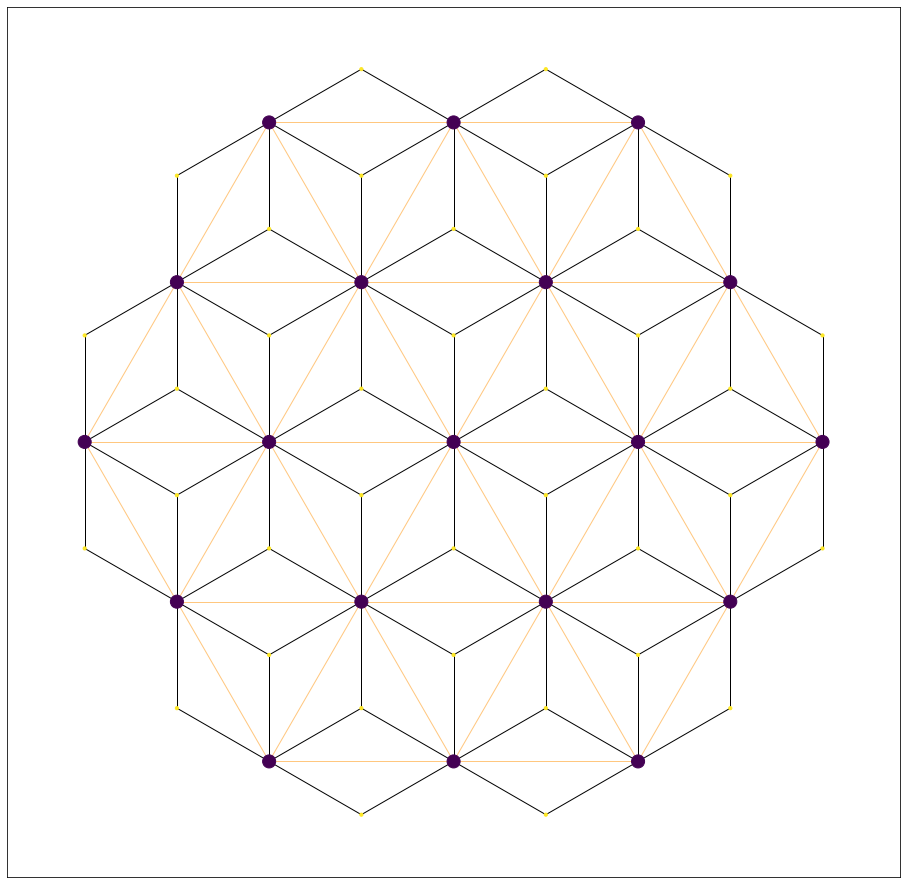
\includegraphics[width=0.8\textwidth]{layout_init.png}
    \caption[Initial layout of the hexagonal lattice flexa sheet]{Initial layout for the flexa sheet projected onto the plane. Cell bodies are shown in large red points and collar boundary vertices are shown in small blue points. Black edges connect cells to collar boundary vertices, and red edges show cell-cell neighbor relations (though these red edges are not physically present). The physical interactions are mediated through the black edges.}
    \label{fig:layout_init}
\end{figure}

\section{Sheet energy} \label{sec:sheet_energy}

\begin{figure}[tbhp]
	\centering
	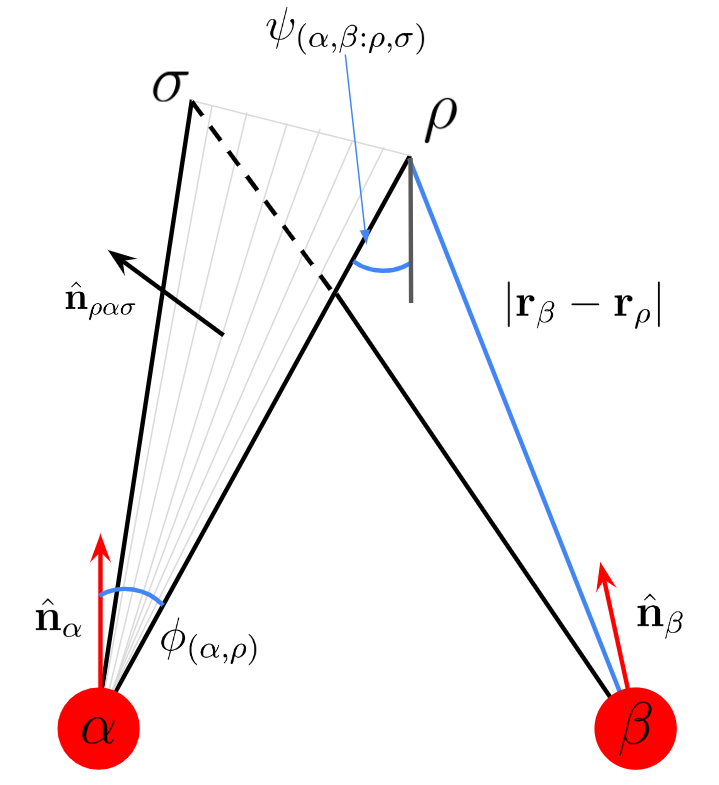
\includegraphics[width=0.6\textwidth]{model.png}
	\caption[Discrete model details]{Detailed view of the discrete model for \textit{C. flexa} sheets shown by the interface between two cells, $\alpha, \beta$ (red), at points $\rho,\sigma$. Cells have unit apicobasal axis vectors $\bh{n}_\alpha, \bh{n}_\beta$, and the plane containing a cell's position $\bm{r}_\alpha$ and two coordinates $\bm{r}_\rho,\bm{r}_\sigma$ belonging to an interface with another cell is defined $\bh{n}_{\rho\alpha\sigma}$. Thin grey microvilli are shown for clarity but not included in the model. The energy (\cref{eq:e}) is defined in terms of angles $\phi_{(\alpha,\rho)}$ and $\psi_{(\alpha,\beta:\rho,\sigma)}$ as well as collar lengths $|\bm{r}_\beta - \bm{r}_\sigma|$.}
	\label{fig:model_details}
\end{figure}

In developing the simplified, discrete model for \textit{C. flexa} as a spatial graph, I aimed to distill the complex physics of collar-collar interactions into a minimum number of sufficient energy terms to capture the sheet bending that we observe experimentally. 
In what follows, I treat edges $(\alpha, \rho)$ between a cell $\alpha$ and collar vertex $\rho$ as straight line collar microvilli and cell pairs, flanking collar pairs $(\alpha, \beta: \rho, \sigma)$ as lines of interactions between the planes given by points $\rho, \alpha, \sigma$ and $\rho, \beta, \sigma$ (\cref{fig:model_details}).
The angles $\phi$ between collar microvilli directions and cell normal vectors and $\psi$ between interfacing collar-cell-collar planes are fully specified by the all cells' coordinates $\{\bm{r}_\alpha\}$, the cells' normal vectors $\{\bm{n}_\alpha\}$ as variables each constrained to have unit length, and the collar interface endpoints $\{\bm{r}_\rho\}$.

Consequently, as detailed in the continuous model description of \cref{ch:2}, I build an energy function $\e = \e(\{\bm{r}_\alpha, \bm{n}_\alpha\}, \{\bm{r}_\rho\})$ that penalises deviations for angles $\phi$ and $\psi$, which describe angles between ($\phi$) collar microvilli and cell normal vectors $\bh{n}_\alpha$, ($\psi$) plane normals $\bh{n}_{\rho\alpha\sigma}, \bh{n}_{\rho\beta\sigma}$, and (sp) collar lengths $|\bm{r}_\alpha - \bm{r}_\rho|$:
\begin{align}
	\e &= \e_\phi + \e_\psi + \e_{\text{sp}}. \label{eq:e}
\end{align}

The terms $\e_\phi$ and $\e_\psi$ capture the energetic penalty incurred by collar bending.
The former results from bending over the length of the collar from the angle formed at the collar base, and the latter captures the bending induced by a neighbouring cell's collars imparting a force.
Moreover, any intrinsic curvature in the collar is captured in the latter term; two filaments each having preferred zero curvature would be in their ground state when the filaments align and cell bodies touch, as in \cref{fig:maxcurv}.
If filaments have intrinsic curvature, the term $\e_\psi$ will encourage distance between cell body positions.
We will see in the following sections that $\e_\phi$ and $\e_\psi$ are functions of all variables $\{\bm{r}_\alpha, \bm{n}_\alpha\}$ and $\{\bm{r}_\rho\}$, while $\e_{\text{sp}}$ is a function only of the spatial coordinates $\{\bm{r}_\alpha\}$ and $\{\bm{r}_\rho\}$.

\subsection{Cell-collar angle energy}
For a physical \textit{C. flexa} cell $\alpha$ with fixed position $\bm{r}_\alpha$ and fixed collar positions $\{\bm{r}_\rho\}_{\rho\subset\alpha}$, we realise that the cell still has freedom in its rotation which we expect will contribute substantially to its energy. 
In other words, there should be an optimal rotation for the cell to minimise its mechanical energy. 
Since we treat \textit{C. flexa} cells as rotationally symmetric above the apicobasal axis, it suffices in our description to assign to each cell $\alpha$ in the graph $\mathfrak{G}$ a unit vector $\bh{n}_\alpha$.
For simplicity, each vector $\bh{n}_\alpha$ is initialised as the unit vector in the direction of $\sum_{\rho\subset\alpha} \vec{\alpha\rho}$, where $\vec{\alpha\rho} = \bm{r}_\rho - \bm{r}_\alpha$.

Defining an energy term on the angle $\phi$ between a cell $\alpha$'s collars and the apicobasal axis $\bh{n}_\alpha$ is done based on descriptions of \textit{Choanoeca} in the literature. 
\citet{brunet2019} describes the change in this angle as the result of exposure to light in \textit{C. flexa}.
Similarly, \citet{ellis1930} characterises the variation in $\phi$ observed in individual cells of \textit{C. perplexa}.

Consequently, we consider an energy term $\e_\phi(\{\bm{r}_\alpha, \bh{n}_\alpha\}, \{\bm{r}_\rho\})$ which penalises devation from a common equilibrium basal collar angle $\phi_0$:
\begin{align}
	\e_\phi(\{\bm{r}_\alpha, \bh{n}_\alpha\}, \{\bm{r}_\rho\}) &= \sum_{(\alpha, \rho)} \left(\phi_{(\alpha, \rho)} - \phi_0 \right)^2. \label{eq:e_phi}
\end{align}
\noindent The sum indicates summation over all cell-collar pairs $(\alpha, \rho)$ in the sheet $\mathfrak{G}$. The angle $\phi_{(\alpha, \rho)}$ is calculated entirely based on the cell normal vector $\bh{n}_\alpha$ and unit vector $\hat{\alpha\rho}$ pointing in the direction of $\bh{r}_\rho - \bh{r}_\alpha$:
\begin{align}
	\phi_{(\alpha, \rho)} &= \arccos \left(\bh{n}_\alpha \cdot \hat{\alpha\rho} \right) = \arccos \left(\bh{n}_\alpha \cdot \frac{\vec{\alpha\rho}}{\left| \vec{\alpha\rho}\right|} \right). \label{eq:phi}
\end{align}

\subsubsection{Optimal cell normal vectors} \label{subsubsec:opt_norm}

No other energy terms will depend on the cell normal vectors $\{ \bh{n}_\alpha \}$, so we ask now what the optimal normal vector for a cell is. Suppose a cell is at position $\bm{r}_\alpha$ with collar vertices at $\bm{r}_\rho$ for $\rho \subset \alpha$. We can determine how the cell orients in order to minimise the collar energy with respect to $\bh{n}_\alpha$. 

For fixed $\alpha$, the cell orientation vector $\bh{n}_\alpha$ is constrained to have unit length. Hence, we solve the constrained optimisation of $\e_\phi$ by solving the Lagrange multiplier problem with multiplier $\lambda$
\begin{align}
    0 &= \frac{\partial \left[ \e_\phi + \lambda\left( \left| \bh{n}_\alpha\right|^2 - 1\right) \right] }{\partial \bh{n}_\alpha} \label{eq:philagrange1} \\
    0 &= \frac{\partial \left[ \e_\phi + \lambda\left( \left| \hat{\bm{n}}_\alpha\right|^2 - 1\right)\right] }{\partial \lambda}. \label{eq:philagrange2}
\end{align}

Using the constraint (solution to \cref{eq:philagrange2}) $| \bh{n}_\alpha |^2 = 1$, we solve 
\begin{align*} 
    \lambda \bh{n}_\alpha &= 2 \sum_{\rho\subset\alpha} \left[ \arccos\left(\hat{\alpha\rho} \cdot \bh{n}_\alpha \right) - \phi_0 \right] \frac{-1}{\sqrt{1 - \left(\hat{\alpha\rho} \cdot \bh{n}_\alpha \right)^2 }} \hat{\alpha\rho} \\
    \lambda &= 2 \left| \sum_{\rho\subset\alpha} \left[ \arccos\left(\hat{\alpha\rho} \cdot \hat{n}_\alpha \right) - \phi_0 \right] \frac{1}{\sqrt{1 - \left(\hat{\alpha\rho} \cdot \hat{n}_\alpha \right)^2 }} \hat{\alpha\rho} \right|.  
\end{align*}
\noindent Then the optimal normal vector solves the transcendental equation 
\begin{align}
    \bh{n}_\alpha &= \frac{\sum_{\rho\subset\alpha} \left[ \arccos\left(\hat{\alpha\rho} \cdot \bh{n}_\alpha \right) - \phi_0 \right] \frac{-1}{\sqrt{1 - \left(\hat{\alpha\rho} \cdot \bh{n}_\alpha \right)^2 }} \hat{\alpha\rho} }{\sum_{\rho\subset\alpha} \left[ \arccos\left(\hat{\alpha\rho} \cdot \bh{n}_\alpha \right) - \phi_0 \right] \frac{1}{\sqrt{1 - \left(\hat{\alpha\rho} \cdot \bh{n}_\alpha \right)^2 }} \hat{\alpha\rho}} \label{eq:optimal_n}
\end{align}

Clearly the cell normal vectors must be computed numerically whenever a cell is interacting with several other cells simultaneously in complicated geometries. 
We can choose to either approximate the normal vectors with a physically reasonable approximation or treat the normal vectors as free arguments to the energy function to be optimised.
I discuss both options below. 

\subsubsection{Approximating cell normal vectors} \label{subsubsec:approx_norm}

There are several options for approximating a cell normal vector $\bh{n}_\alpha$ based on positions $\bm{r}_\alpha$ and $\{ \bm{r}_\rho\}_{\rho\subset\alpha}$.
The simplest option is to let $\bh{n}_\alpha$ be the unit vector in the direction $\sum_{\rho\subset\alpha}\vec{\alpha\rho}$. 
This approach has the benefit that collar vertices farther from $\bm{r}_\alpha$ are weighted more in the cell normal vector, agreeing with the intuition that a more distant collar interaction demands more cell rotation to accommodate it. 
However, I found that this approach results in unreasonable cell normal vectors for boundary cells as defined in $\mathfrak{G}$ since boundary cells do not have a full ring of boundary collar vertices. 
For this approach to work, $\mathfrak{G}$ would need to include several more collar vertices which do not describe interactions between cells and add unnecessary complexity.
In application, I found that the boundary cell effect of this choice of $\bh{n}_\alpha(\bm{r}_\alpha, \{\bm{r}_\rho\}_{\rho\subset\alpha})$ substantially affected boundary collar vertex positions after energy equilibration and the overall energy landscape as a function of equilibrium angles $\phi_0, \psi_0$. 

When initialising a flat sheet, the above averaging approach also does not agree with intuition, since it results in boundary cell normal vectors that do not point in the same direction as normal vectors for cells not on the sheet boundary (\cref{fig:layout_init}). Instead, when a sheet lies flat in the $xy$-plane, it is expected that all vectors $\bh{n}_\alpha$ point in the $+\hat{z}$ direction provided that collars are above cells in $\bm{z}$. 
A viable alternative is to define $\bh{n}_\alpha$ by taking a plane approximation to cell $\alpha$'s collar vertices. 
The normal vector to this plane oriented away from the cell defines a normal vector that agrees with intution and supports calculating normals for a non-coplanar set of collar vertices.

The plane approximation approach is easiest achieved using ordinary least squares. 
Briefly, we approximate $\hat{r}_{\rho 3} = (r_{\rho 1}, r_{\rho 2}) \cdot (\beta_1, \beta_2) + \beta_0$ and minimise the sum of squared residuals $\sum_{\rho\subset\alpha} (\hat{r}_{\rho 3} - r_{\rho 3})^2$ with respect to $\beta_0, \beta_1, \beta_2$. 
The normal vector of the plane approximation is then $(\hat{\beta}_1, \hat{\beta}_2, -1)$ up to normalisation and multiplication by $-1$.\footnote{The notation here is chosen to be consistent with that typically used in ordinary least squares, hence the hatted values indicate an approximation rather than vector normalisation as I use otherwise.} 
Although the gradient of the energy \cref{eq:e} can be computed in this approximation, I found that it resulted in frequent numerical instabilities.

Due to the lack of a suitable approximation to the apicobasal axis vectors $\bh{n}_\alpha$ in terms of the cell $\alpha$'s position and its collar vertices' positions, I instead let these vectors be free variables.

\subsection{Collar-collar interface angle energy} \label{subsec:e_psi}

As in \cref{ch:2}, the goal is to produce sheet curvature with the angle $\psi$ that two cells' collars make at their interface. As in \cref{subsubsec:bdary_verts}, I calculate the angle between planes defined by two cells $\alpha, \beta$ and their mutual flanking collar vertices $\rho, \sigma$ with
\begin{align}
	\psi_{(\alpha, \beta: \rho, \sigma)} &= \frac{\pi}{2} - \frac{1}{2}\arccos \left(\bh{n}_{\rho\alpha\sigma} \cdot \bh{n}_{\rho\beta\sigma} \right). \label{eq:psi}
\end{align}
\noindent The normal vectors $\bh{n}_{\rho\alpha\sigma}$ for a plane given by points $\rho, \alpha, \sigma$ must have a systematically defined orientation, as they can point in either direction $\pm (\bm{r}_\rho - \bm{r}_\alpha) \times (\bm{r}_\sigma - \bm{r}_\alpha)$. 
In the geometry used to define $\psi$ in \cref{eq:psi}, the collar-cell-collar normal vectors are assumed to be pointing in the direction of the cells' flagella. 
With the simplifying assumption that the cell normal always points in the inside of the collar, we have that the collar-cell-collar normals must take orientation to align with their corresponding cell normals. 
Consequently, I let $\bm{n}_{\rho\alpha\sigma}' = \vec{\alpha\rho} \times \vec{\alpha\sigma}$ and set $\bh{n}_{\rho\alpha\sigma} = \sgn (\bm{n}_{\rho\alpha\sigma}' \cdot \bh{n}_\alpha) \bh{n}_{\rho\alpha\sigma}'$.
Here $\sgn$ is the sign operator: $\sgn(x) = 1$ if $x \geq 0$ and $\sgn(x) = -1$ if $x < 0$.

Defining $\bh{n}_{\rho\alpha\sigma}$ in this way makes it dependent on the cell normal vectors $\bh{n}_\alpha$. 
However, when minimising the energy, I work to develop methods such that $\sgn (\bh{n}_{\rho\alpha\sigma} \cdot \bh{n}_\alpha)$ remains constant (see later \cref{eq:e_varphi}). 
This corresponds to ensuring that no collar vertices cross through each other (corresponding to microvilli crossing over each other) and that the cell normal vectors remain pointing inside the collars.
Hence, I effectively treat the effect of $\bh{n}_\alpha$ on a collar-cell-collar normal vector $\bh{n}_{\rho\alpha\sigma}$ to be constant.

With a common equilibrium collar-collar interface angle $\psi_0$ (as all cells are assumed equal in their mechanical properties), I express the energy $\e_\psi$ 
\begin{align}
	\e_\psi &= k_\psi \sum_{(\alpha, \beta: \rho, \sigma)} (\psi_{(\alpha, \beta: \rho, \sigma)} - \psi_0)^2. \label{eq:e_psi}
\end{align}

\subsection{Collar length}

To provide sufficient flexibility to sheets through collar microvilli, I introduce an energy term $\e_{\text{sp}}$ defined by 
\begin{align}
	\e_{\text{sp}} &= k_{\text{sp}} \sum_{(\alpha, \rho)} \left| \vec{\alpha\rho} - \ell_{0\alpha\rho} \right|^2, \label{eq:e_sp}
\end{align}
\noindent where $\ell_{0\alpha\rho}$ is an equilibrium length for edge $(\alpha, \rho)$. The sum indicates summation over all cell, collar pairs $(\alpha, \rho)$ in the sheet $\mathfrak{G}$.

All cells are assumed to take identical properties, so all values $\ell_{0\alpha\rho}$ are set to a constant $\ell_0$ unless indicated otherwise. 
When done so, we find that $\phi_0, \psi_0$, and $\ell_0$ allow us to calculate a natural length scale for the problem, $1/H_0$ (\cref{eq:h0}).

When interested in sheets with constrained collar length, we may either take a numerical approach or exploit the above energy term by setting $k_{\text{sp}}$ to a large value. 

\section{Minimising sheet energy} \label{sec:minimise_energy}

The sheet energy $\e(\{\bm{r}_\gamma \}_{\gamma \in \mathfrak{G}}, \{\bm{n}_\alpha\}_{\alpha\in G})$ (\cref{eq:e}) is parameterised over the cell and collar boundary vertex coordinates as well as the free apicobasal axis unit vectors $\bm{n}_\alpha$ for cell bodies $\alpha$.
When sheet topology is left fixed, the summations in \cref{eq:e_phi,eq:e_psi,eq:e_sp} remain unchanged.

Minimisations of \cref{eq:e} using a numerical optimisation routine were suitable in simple, small systems. 
Greater deflections out of the plane or larger sheet topologies resulted in more frequent numerical instabilities, however.
Numerical instability arises in solving \cref{eq:e} due to the discontinuities in $\e_\psi$. 
Since collar-cell-collar normal vectors $\bh{n}_{\rho\alpha\sigma}$ are oriented using $\vec{\alpha\rho} \times\vec{\alpha\sigma}$, where the order of the cross product is fixed, the change in sign when $\bm{r}_\rho$ and $\bm{r}_\sigma$ cross each other gives a discontinuity in the calculation of angles $\psi_{(\alpha,\beta:\rho,\sigma)}$. 

Since collars are not explicitly restricted from crossing each other here, this model must be solved within confined region of its state space.
I achieve this by performing gradient descent, which physically translates to integrating the forces on each vertex under equal linear isotropic drag.

All code written and used in this chapter is available online at \url{https://github.com/adkonk/flexa}.

\subsubsection{Flat sheet as a solution} \label{subsubsec:flat}

A flat sheet generated with a hexagonal lattice has a regular structure that makes $\phi_{\alpha\rho} = \phi_0$, $\psi_{(\alpha,\beta:\rho\sigma}) = \psi_0$, $|\bm{r}_\alpha - \bm{r}_\rho| = \ell_0$ for all cell-collar pairs $(\alpha,\rho)$ and collar-collar interfaces $(\alpha,\beta:\rho,\sigma)$. 
Consequently, all terms in $\e$ (\cref{eq:e}) are zero.
Since $\e_\phi$ and $\e_\psi$ are nonnegative, the flat sheet is a stable solution for appropriate $\phi_0, \psi_0$. 

Moreover, given \cref{eq:h0} describing sheet curvature in terms of $\phi_0, \psi_0$ and the geometry of collar interactions (\cref{fig:hpsi}), we expect that any pair $(\phi_0, \psi_0)$ where $\phi_0 = \psi_0$ will give a zero energy, flat sheet.
A landscape of minimum sheet energies over several pairs $(\phi_0, \psi_0)$ is expected to feature a minimum energy valley along the diagonal.

% \subsubsection{Solving sheet shape}
% 
% Numerical optimisation: sensitivity issues and initial conditions
% 
% Derive the gradient
% 
% Describe how to compute the gradient in an efficient way
% 
% \subsection{Graph topology}
% For hexagonal lattice start, we 
% 
% Call back to section \ref{sec:c_1d}

\subsection{Energy gradient descent} \label{subsec:grad_desc}

The goal in using gradient descent is to explicitly calculate the gradients $\partial \e / \partial \bm{r}_\gamma$ of the energy with respect to all coordinate vectors $\bm{r}_\gamma$ and incrementally take small steps in the reverse direction. 

Although gradient descent in several contexts is criticised for being slow and by nature prone to be trapped in local minima, in the context of modeling \textit{C. flexa} sheets it is preferable to a black box optimisation routine. 
Calculating the gradient analytically amounts to calculating the forces on all coordinates, and taking incremental steps in the direction of the negative gradient amounts to forward integrating the force $F_\gamma = - \partial\e/\partial\bm{r}_\gamma$. 
As in \cref{ch:2}, I assume linear drag such that $\zeta d\bm{r}_\gamma/dt = -\partial\e/\partial\bm{r}_\gamma$. 
Consequently, I gain access to the dynamics induced by the simplified model that I describe above. 
Moreover, the susceptibility of this approach to be trapped in local minima is ideal not only from an energetic perspective, but also from a numerical one: by taking incremental steps in a direction known to decrease the energy, any increases in energy indicate too large a step size or a discontinuous jump in the energy from collar vertices crossing each other.

In contrast to a numerical optimisation routine, gradient descent requires substantial explicit calculation. Moreover, the algorithm requires tuning in the step size and relative decrease in energy tolerance at which to decide the algorithm has terminated. 

\subsection{Deriving the gradient}

The linearity of the gradient permits us to take the gradient term-by-term in \cref{eq:e}.
For energy function $\e_\phi(\{ \bm{r}_\alpha, \bm{n}_\alpha\}, \{\bm{r}_\rho\})$, I find that the gradient $\partial \e_\phi / \partial \bm{r}_\gamma$ is given by 
\begin{align}
	\frac{\partial\e_\phi}{\partial\bm{r}_\gamma} &= \sum_{(\alpha,\rho)} \frac{-(\phi_{(\alpha,\rho)} - \phi_0)}{\sqrt{1-(\bh{n}_\alpha \cdot \hat{\alpha\rho})^2}} \left(\frac{\partial\hat{\alpha\rho}}{\partial\bm{r}_\gamma} \cdot \bh{n}_\alpha \right), \label{eq:grad_phi}
\end{align}
\noindent where for vectors $\bm{a}, \bm{b}$ I denote $(\partial\bm{a}/\partial\bm{b})_{ij} = \partial\bm{a}_j /\partial\bm{b}_i$.
\Cref{eq:grad_phi} applies over indices $\gamma$ describing both cell bodies and collar-collar interface points.
Calculating equation \cref{eq:grad_phi} is completed with
\begin{align}
	\frac{\partial \hat{\alpha\rho}_j}{\partial\bm{r}_{\gamma i}} &= \frac{\delta_{\gamma\rho}-\delta_{\gamma\alpha}}{|\vec{\alpha\rho}|} \left[\delta_{ij} - (\vec{\alpha\rho})_i(\vec{\alpha\rho})_j \right], \label{eq:dap_dr}
\end{align}
where $\delta_{\gamma\rho}$ is an indicator function for equality between $\gamma$ and $\rho$. 

Equations \cref{eq:grad_phi,eq:dap_dr} can be rearranged to efficiently calculate $\partial\e_\phi/\partial\bm{r}_\gamma$ with matrix multiplication by grouping terms dependent on $\gamma$, given an ordering of indices $(\alpha,\rho)$:
\begin{align}
	\frac{\partial\e_\phi}{\partial\bm{r}_{\gamma i}} &= \sum_{(\alpha,\rho)} \underbrace{(\delta_{\gamma\rho} - \delta_{\gamma\alpha})}_{A_{\gamma,(\alpha,\rho)}} \underbrace{\frac{-(\phi_{(\alpha,\rho)} - \phi_0)}{\sqrt{1-(\bh{n}_\alpha \cdot \hat{\alpha\rho})^2} |\vec{\alpha\rho}|} \left(\bh{n}_\alpha - \hat{\alpha\rho} (\bh{n}_\alpha \cdot \hat{\alpha\rho}) \right)}_{B_{(\alpha,\rho), i}}, \label{eq:grad_phi_mx}
\end{align}
where $A$ and $B$ are matrices with entries enclosed in the braces. 
The remaining gradient terms \cref{eq:grad_psi} can also be rearranged as matrix multiplications to speed up calculation.

As discussed in \ref{subsec:e_psi}, an angle $\psi_{(\alpha, \beta: \rho, \sigma)}$ for a cell-cell interface depends in a piecewise constant way on the cells' normal vectors. While the angles are consequently only piecewise differentiable, gradient descent makes the reasonable assumption that there will not be any discontinuities in $\e_\psi$ for sufficiently small steps in the direction of the negative gradient. The below expression for $\partial \e_\psi / \partial \bm{r}_\gamma$ assumes that the sign of $\bh{n}_\alpha \cdot (\vec{\alpha\rho}\times \vec{\alpha\sigma})$ remains constant.
\begin{align}
	\frac{\partial \e_\psi}{\partial \bm{r}_\gamma} &= k_\psi \sum_{(\alpha,\beta: \rho,\sigma)} \frac{\left(\psi_{(\alpha,\beta:\rho,\sigma)} - \psi_0 \right)}{2\sqrt{1 - (\bh{n}_{\rho\alpha\sigma}\cdot \bh{n}_{\rho\beta\sigma})^2}} \left(\bh{n}_{\rho\alpha\sigma} \cdot \frac{\partial \bh{n}_{\rho\beta\sigma}}{\partial \bm{r}_\gamma} + \bh{n}_{\rho\beta\sigma} \cdot \frac{\partial \bh{n}_{\rho\alpha\sigma}}{\partial \bm{r}_\gamma} \right) \nonumber \\
	\bh{n}_{\rho\alpha\sigma} \cdot \frac{\partial \bh{n}_{\rho\beta\sigma}}{\partial \bm{r}_\gamma} &= \frac{\sgn \left(\vec{\beta\rho} \times \vec{\beta\sigma} \cdot \bh{n}_\beta \right)}{|\vec{\beta\rho} \times \vec{\beta\sigma}|} \left[ \left(\frac{\bh{n}_{\rho\alpha\sigma} \cdot \vec{\beta\rho}\times\vec{\beta\sigma}}{|\vec{\beta\rho}\times\vec{\beta\sigma}|^2} \vec{\beta\rho}\times\vec{\beta\sigma} - \bh{n}_{\rho\alpha\sigma} \right) \right. \nonumber \\
	&\qquad\qquad\qquad \left. \times \left( (\delta_{\gamma\rho} - \delta_{\gamma\beta}) \vec{\beta\sigma} - (\delta_{\gamma\sigma} - \delta_{\gamma\beta}) \vec{\beta\rho} \right) \right] \label{eq:grad_psi}
\end{align}

The gradient $\partial \e_{\text{sp}} / \partial \bm{r}_\gamma$ is given by the linear spring force 
\begin{align}
	\frac{\partial\e_{\text{sp}}}{\partial\bm{r}_\gamma} &= k_{\text{sp}} \sum_{(\alpha,\rho)} \left(\delta_{\alpha\gamma} - \delta_{\rho\gamma} \right)\vec{\alpha\rho} \label{eq:grad_sp}
\end{align}
which is simply Hooke's law.

\subsection{Forward integration} \label{subsec:forward_int}

Integrating the gradient given by equations \cref{eq:grad_phi,eq:grad_psi,eq:grad_sp} with linear local drag produces the dynamics of sheet bending as in \cref{fig:dynamics}. 
We can numerically integrate using gradient descent with finite step size $\Delta t$ and drag coefficient $\zeta$.
\mynote{discuss the equilibrium states}
\begin{align}
	\bm{r}_\gamma(t+\Delta t) &= \bm{r}_\gamma (t) - \zeta \Delta t \frac{\partial \e}{\partial \bm{r}_\gamma}. \label{eq:grad_desc_r}
\end{align}
We can factor $k_\phi$ from each of \cref{eq:grad_phi,eq:grad_psi,eq:grad_sp} to use step $\zeta k_\phi \Delta t$ in \cref{eq:grad_desc_r} and describe the energy in \cref{eq:e} with $(1, k_\psi / k_\phi, k_{\text{sp}} / k_\phi)$.
With one of three energy constants only serving to affect the timescale, only the remaining two are free.
I set $k_\psi / k_\phi = 2$ and $k_{\text{sp}} / k_\phi = 5$ for the results in this work, though the results were not found to qualitatively differ significantly for small differences in these constants.\footnote{A value of $2$ was chosen since each cell-cell interface is only counted once in \cref{eq:e_psi}, despite two collar microvilli being represented at each interface.}

When treating the normal vectors $\bh{n}_\alpha$ as free variables, we must modify our force equilibration algorithm to maintain the constraint that $| \bh{n}_\alpha |^2 = 1$. 
An intuitive option is to step in the direction of the negative gradient and normalise the intermediate vectors at each step:

\begin{align}
	\bm{n}_\alpha(t+\Delta t) &= \bh{n}_\alpha(t) - \zeta \Delta t \frac{\partial \e}{\partial \bh{n}_\alpha} \label{eq:grad_desc_n1}\\
	\bh{n}_\alpha(t+\Delta t) &= \frac{\bm{n}_\alpha(t+\Delta t)}{\bm{n}_\alpha(t+\Delta t)}. \label{eq:grad_desc_n2}
\end{align}

Equivalently, since for a sufficiently small step size the nearest point on the constraint set $|\bh{n}_\alpha|^2=1$ to $\bm{n}_\alpha(t+\Delta t)$ is unique, we may re-express \cref{eq:grad_desc_n2} with $\bh{n}_\alpha(t + \Delta t) = \arg \min_{|\bh{n}_\alpha|^2 = 1} |\bh{n}_\alpha - \bm{n}_\alpha(t+\Delta t)|$.
Expressed in this way, we see that the update for $\bh{n}_\alpha$ expressed in \cref{eq:grad_desc_n1,eq:grad_desc_n2} is exactly the projected gradient descent algorithm and we expect it to converge \citep{eicke1992}.
Since the normal component of $\partial \e / \partial \bh{n}_\alpha$ to the constraint set $|\bh{n}_\alpha|^2 = 1$ at step $t$ does not affect $\bh{n}_\alpha(t + \Delta t)$, we can interpret \cref{eq:grad_desc_n1,eq:grad_desc_n2} as taking a step in the direction of the tangent space to the constraint set that reduces $\e$ the most.

\begin{landscape}
\begin{figure}[p]
	\centering
	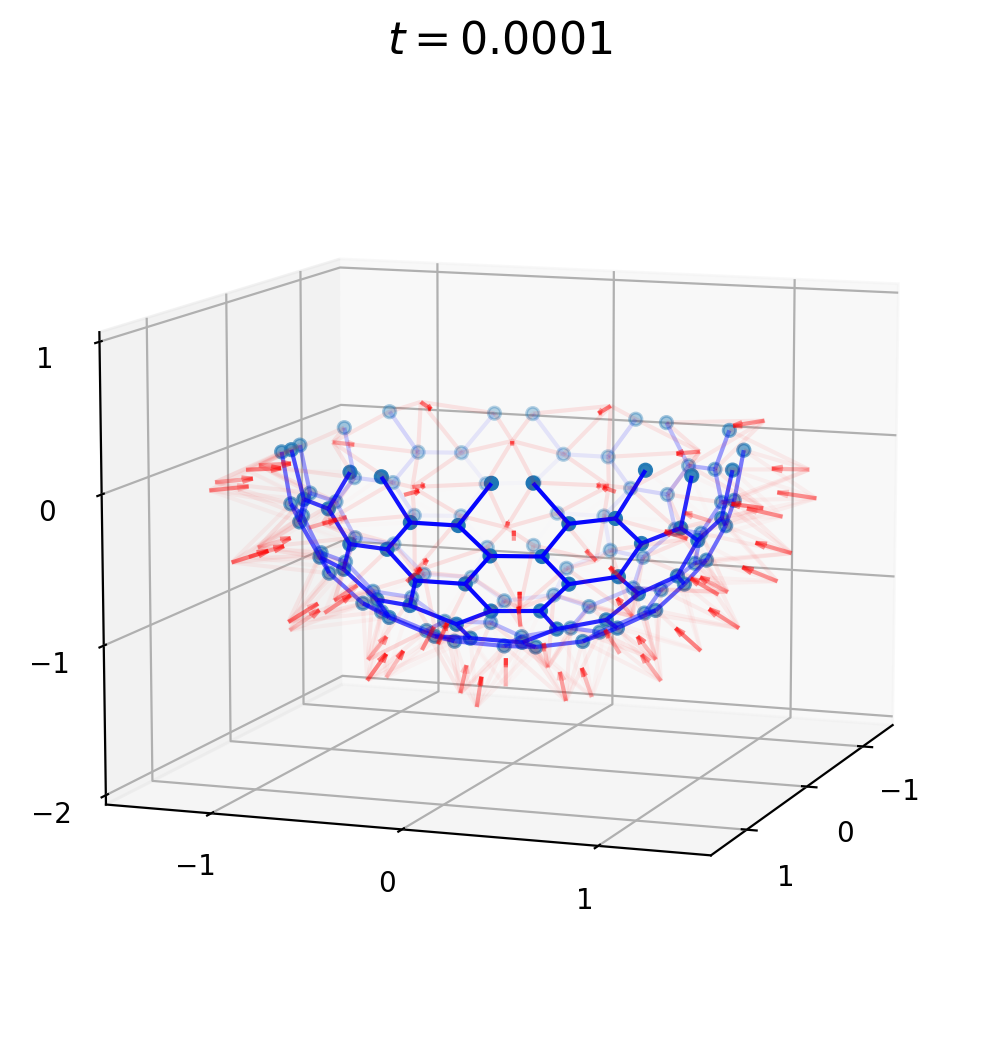
\includegraphics[width=0.4\textheight]{dynamics/00000.png}
	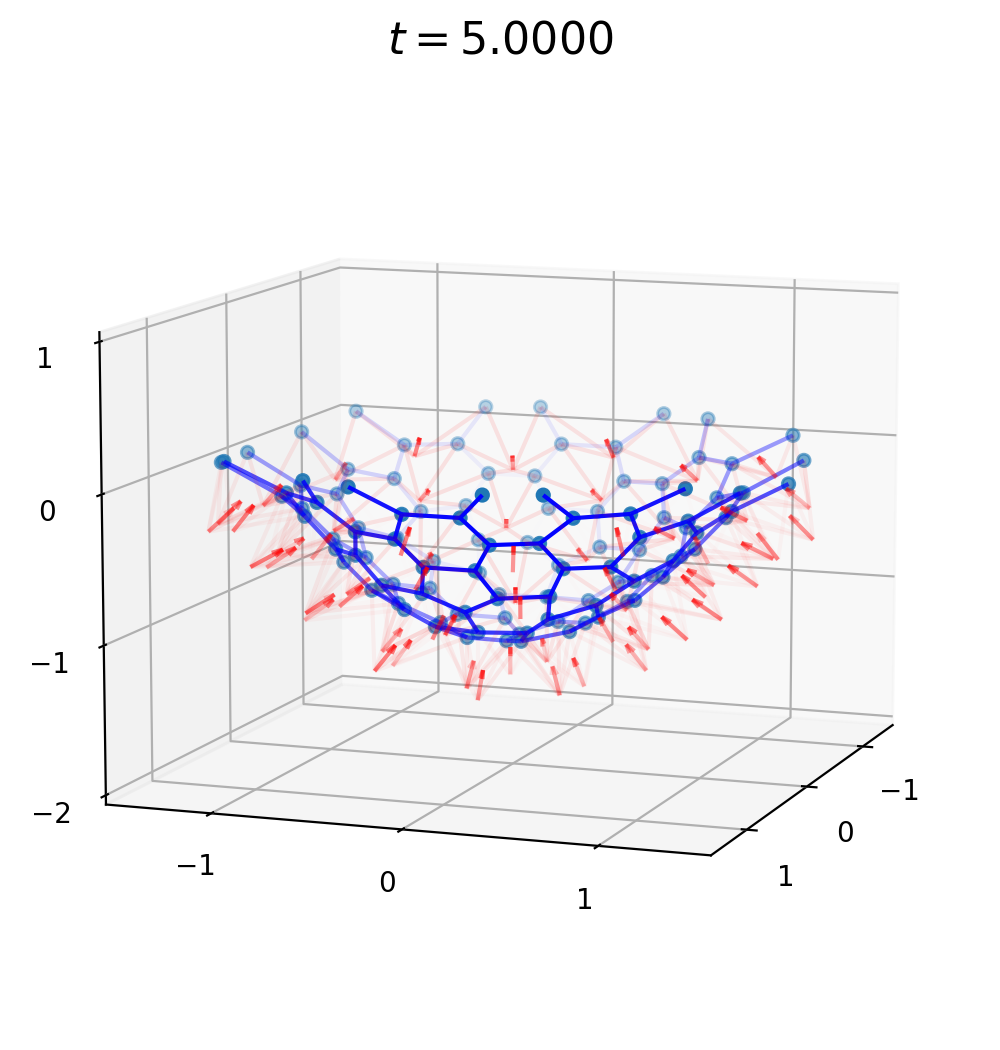
\includegraphics[width=0.4\textheight]{dynamics/02000.png}
	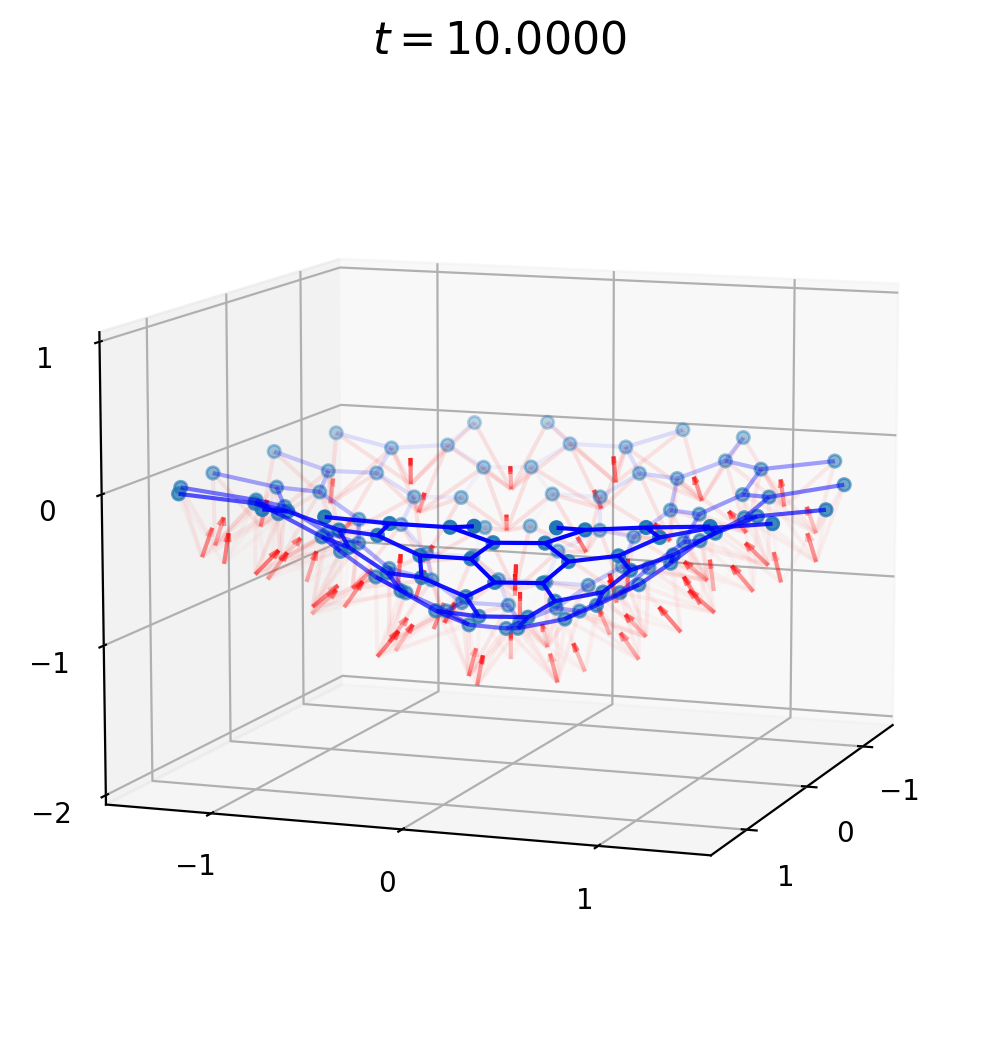
\includegraphics[width=0.4\textheight]{dynamics/04000.png}
	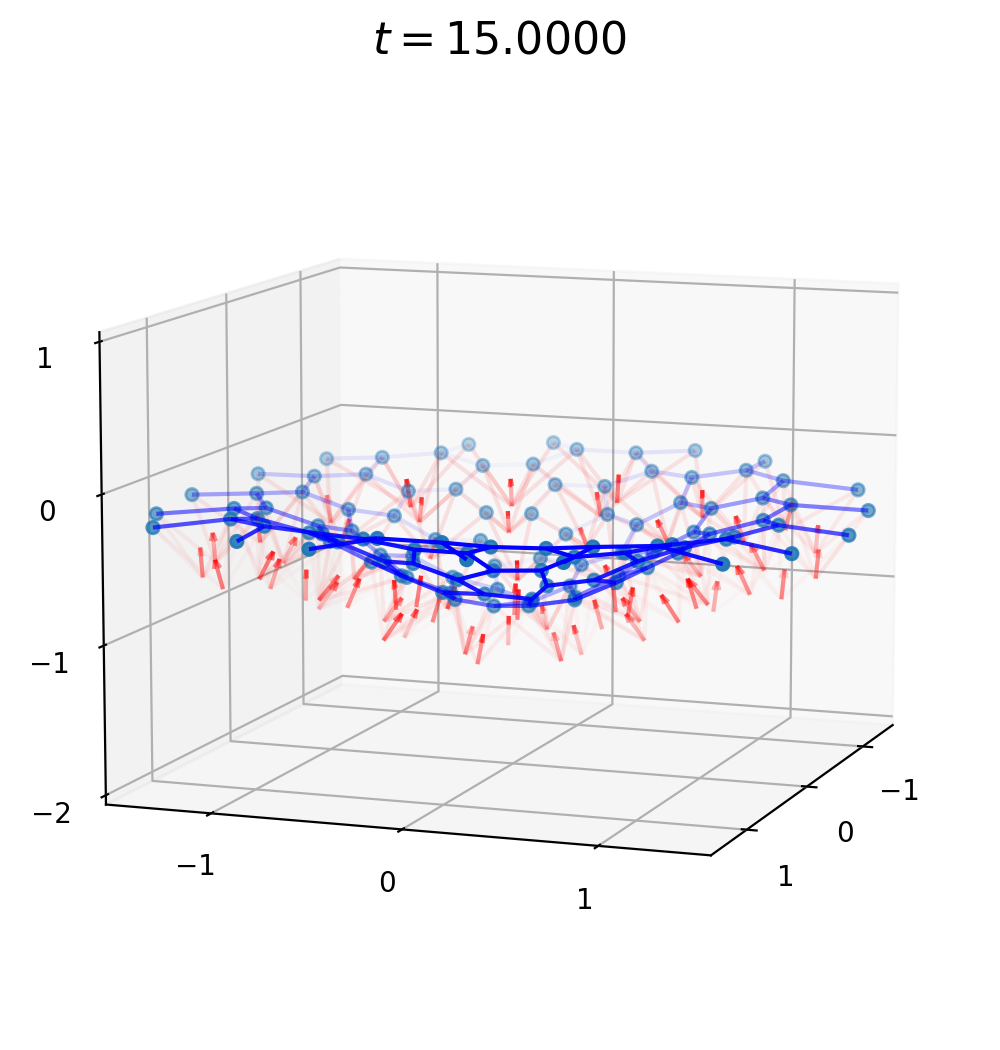
\includegraphics[width=0.4\textheight]{dynamics/06000.png}
	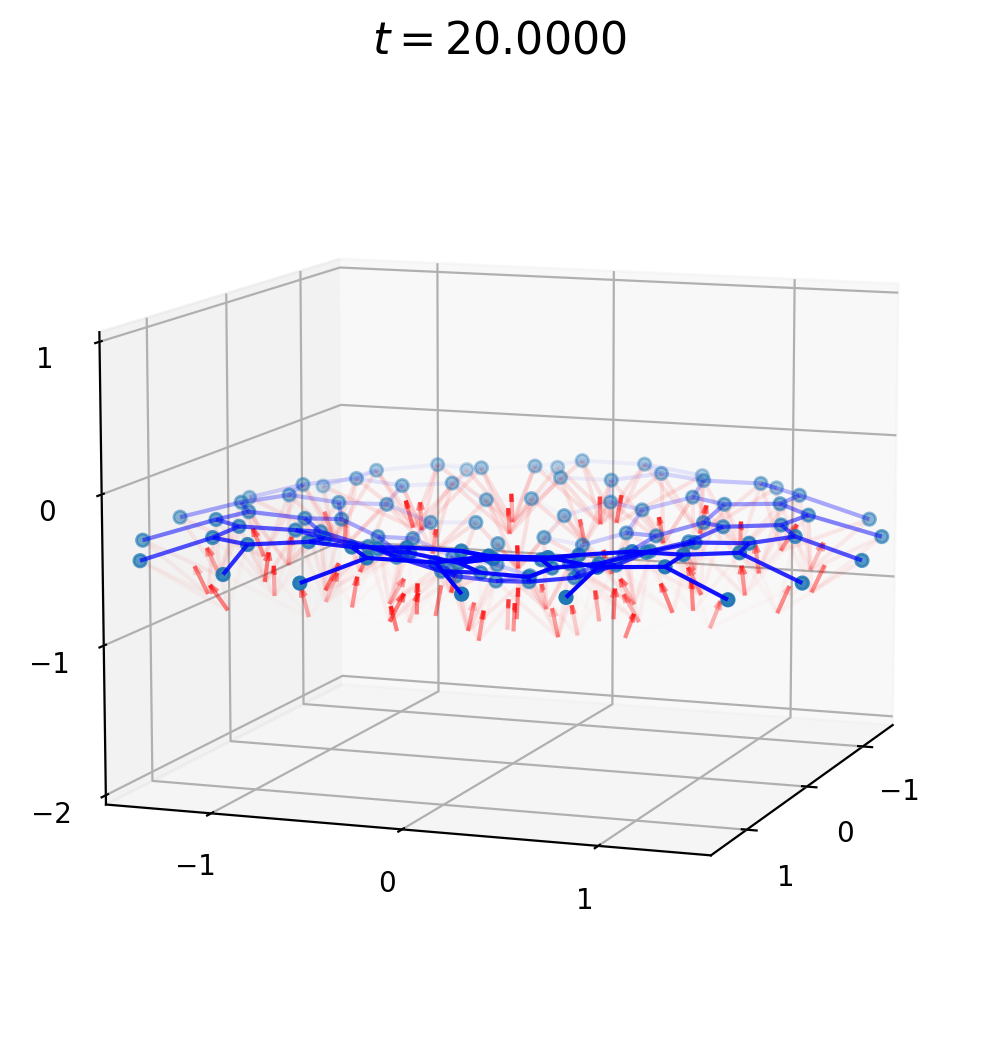
\includegraphics[width=0.4\textheight]{dynamics/08000.png}
	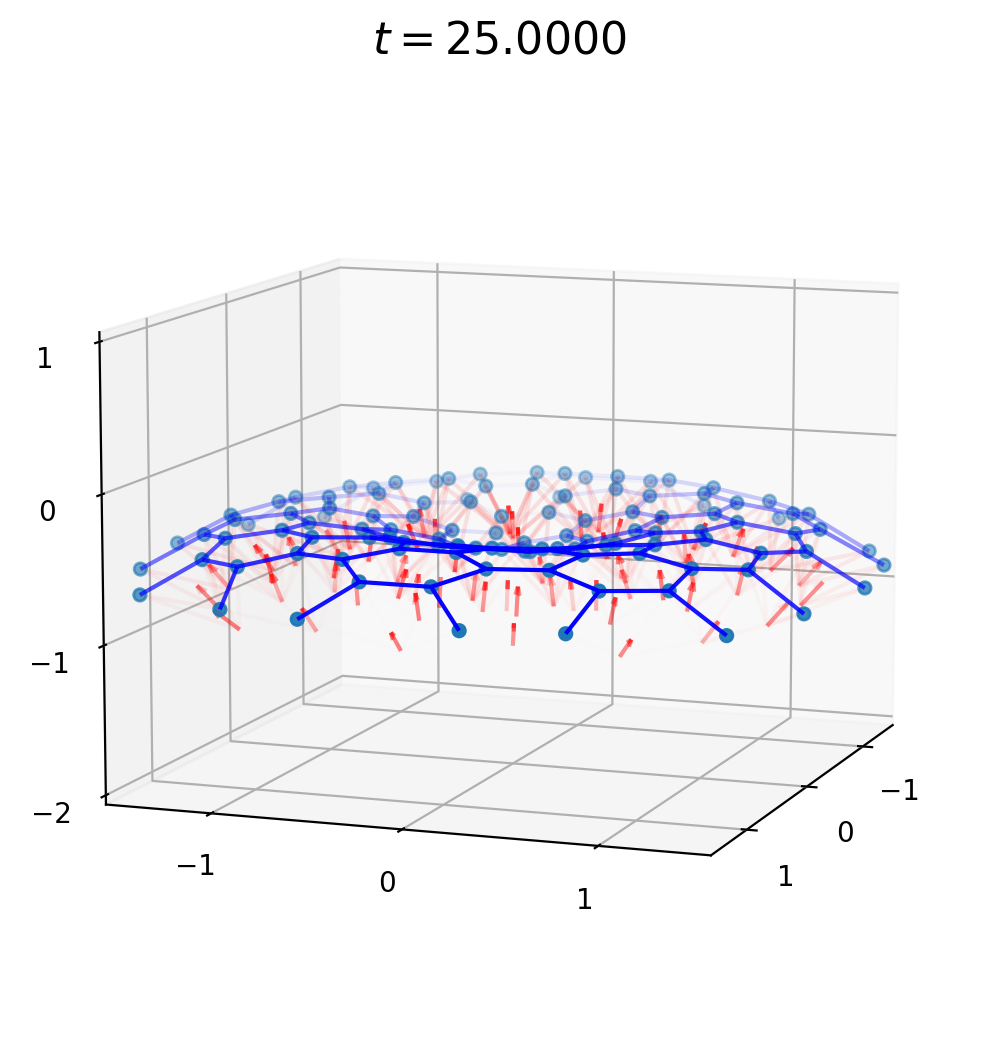
\includegraphics[width=0.4\textheight]{dynamics/10000.png}
	\caption[Gradient descent equilibration and dynamics of sheet inversion]{Dynamics of sheet inversion under linear drag in the transition from $(\phi_0, \psi_0)=(0.55, 0.65)$ to $(0.71,0.41)$ demonstrating projected gradient descent using \cref{eq:grad_desc_r,eq:grad_desc_n1,eq:grad_desc_n2}.}
	\label{fig:dynamics}
\end{figure}
\end{landscape}

While the forward integration works well for small sheets with simple graph topologies, I found that some equilbrium angles $\phi_0, \psi_0$ caused some sheets to strain to such an extreme that collar vertices would cross through each other. 
The resulting increase in energy comes from the discontinuous sign function in the definition of $\psi$ (\cref{eq:psi}), and collar vertices cross over each other due to too large of a step size $\Delta t$. 
While adaptively decreasing the step size is a viable option, it would substantially slow the equilibration algorithm.  
Instead, I introduced an additional term to the energy $\e_\varphi$ based on the angles $\varphi_{\rho\alpha\sigma}$ formed by each cell $\alpha$ and its adjacent pairs of collar vertices $\rho,\sigma$ when projected onto the plane defined by the cell normal $\bh{n}_\alpha$ (\cref{fig:varphi}):
\begin{align}
	\e_\varphi &= k_\varphi \sum_{(\alpha,\beta:\rho\sigma)} \left(\varphi_{\rho\alpha\sigma} - \varphi_{0\rho\alpha\sigma} \right)^2, \label{eq:e_varphi}
\end{align}
\noindent where $\varphi_{0\rho\alpha\sigma}$ is an equilibrium projected collar-cell-collar angle for each triple. 
Each angle $\varphi_{0\rho\alpha\sigma}$ is set to the actual value that is evaluated at the initial sheet geometry.
Unless specified otherwise, the constant $k_\varphi$ is set to $0.3k_\phi$, which was qualitatively found to be a reasonable balance between preventing numerical instability and minimally interfering in the structure transition.
It is worth noting that $\e_\varphi$ has physical interpretation as penalising collars that do not extend radially outward relative to the cell's normal vector.

\begin{figure}
	\centering 
	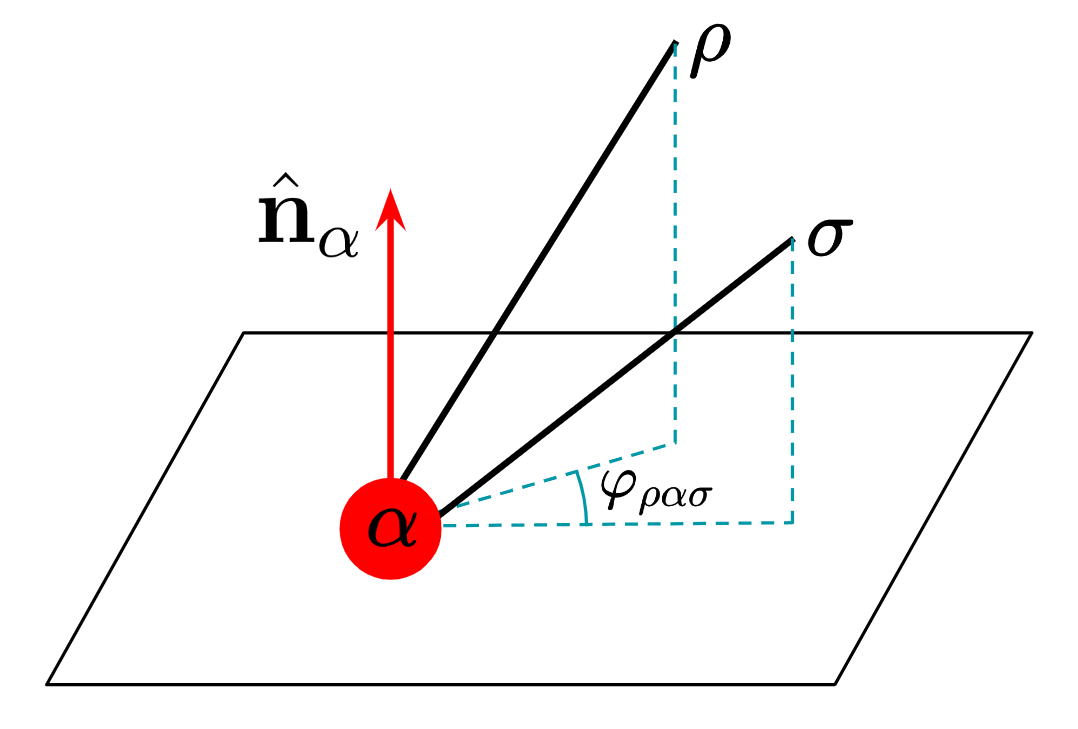
\includegraphics[width=0.5\textwidth]{varphi.png}
	\caption{Geometry for calculating $\varphi_{\rho\alpha\sigma}$.}
	\label{fig:varphi}
\end{figure}

The angles $\varphi_{\rho\alpha\sigma}$ are calculated similarly to $\phi, \psi$ (\cref{eq:phi,eq:psi}),
\begin{align}
	\varphi_{\rho\alpha\sigma} &= \arccos \left[\vec{\alpha\rho}_\| \cdot \vec{\alpha\sigma}_\| \right], \label{eq:varphi}
\end{align}
\noindent where $\vec{\alpha\rho}_\|$ is the projection of $\vec{\alpha\rho}$ onto the plane defined by normal $\bh{n}_\alpha$ and position $\bm{r}_\alpha$:
\begin{align*}
\vec{\alpha\rho}_{\|} &= \vec{\alpha\rho} - (\vec{\alpha\rho} \cdot \bh{n}_\alpha) \bh{n}_\alpha.
\end{align*}

% The gradient of $\e_\varphi$ is given by 
% 
% \begin{align}
% 	todo \label{eq:grad_varphi}
% \end{align}

Note that 
\begin{align}
	\bm{0} &= \sum_\gamma \frac{\partial}{\partial\bm{r}_\gamma} \e \label{eq:force_zero}
\end{align}
since all forces are generated internally.
Moveover, \cref{eq:force_zero} holds individually for each term in the energy (\cref{eq:e}), which is evident by the indicator functions in \cref{eq:grad_phi,eq:grad_psi,eq:grad_sp}.

\subsection{Exploring the energy landscape} \label{subsec:landscape}

With the ability to study discrete sheet equilibrium geometries and dynamics, we are prepared to evaluate a mechanism for \textit{C. flexa} folding and inversion. 
Based on the two collar angle states observed in \citet{brunet2019}, a reasonable model would be to assume relaxed-state equilibrium angles $\phi_{\text{in}}, \psi_{\text{in}}$ and a different set of active-state angles $\phi_{\text{out}}, \psi_{\text{out}}$ with instantaneous transition between the two states. 
The rapid change in individual cell behavior and expected gradual sheet shape change expected from opposing cell-cell interactions align with our expectations from observations \citet{brunet2019}. 

Although we cannot access true values for the equilibrium angles, modeling \textit{C. flexa} sheets numerically provides the opportunity to explore the entire energy landscape. 
For sheets generated with a regular hexagonal lattice, we observe the expected diagonal valley where energy in minimised in the energy landscape since the sheet is expected to be flat along those pairs $(\phi_0, \psi_0)$ (\cref{fig:landscape_flat}) (\cref{subsubsec:flat}).
Substantial sheet deformation and bending is evidently not sufficient to overcome the change in terms in the energy function. 
The increases in energy when the equilibrium angles are most disparate can be interpreted as collar microvilli stretching or compressing to accommodate sheet bending or a difference in the bending at each cell from the preferred state. 
For example, cells at either the centre nor boundary in a bent sheet (\cref{fig:landscape_flat}, bottom-right or top-left) must contribute a positive contribution to $\e$ since they do not have the symmetric bending at all collar microvilli prescribed by \cref{eq:e_phi,eq:e_psi,eq:e_sp}.

\begin{figure}
	\centering
	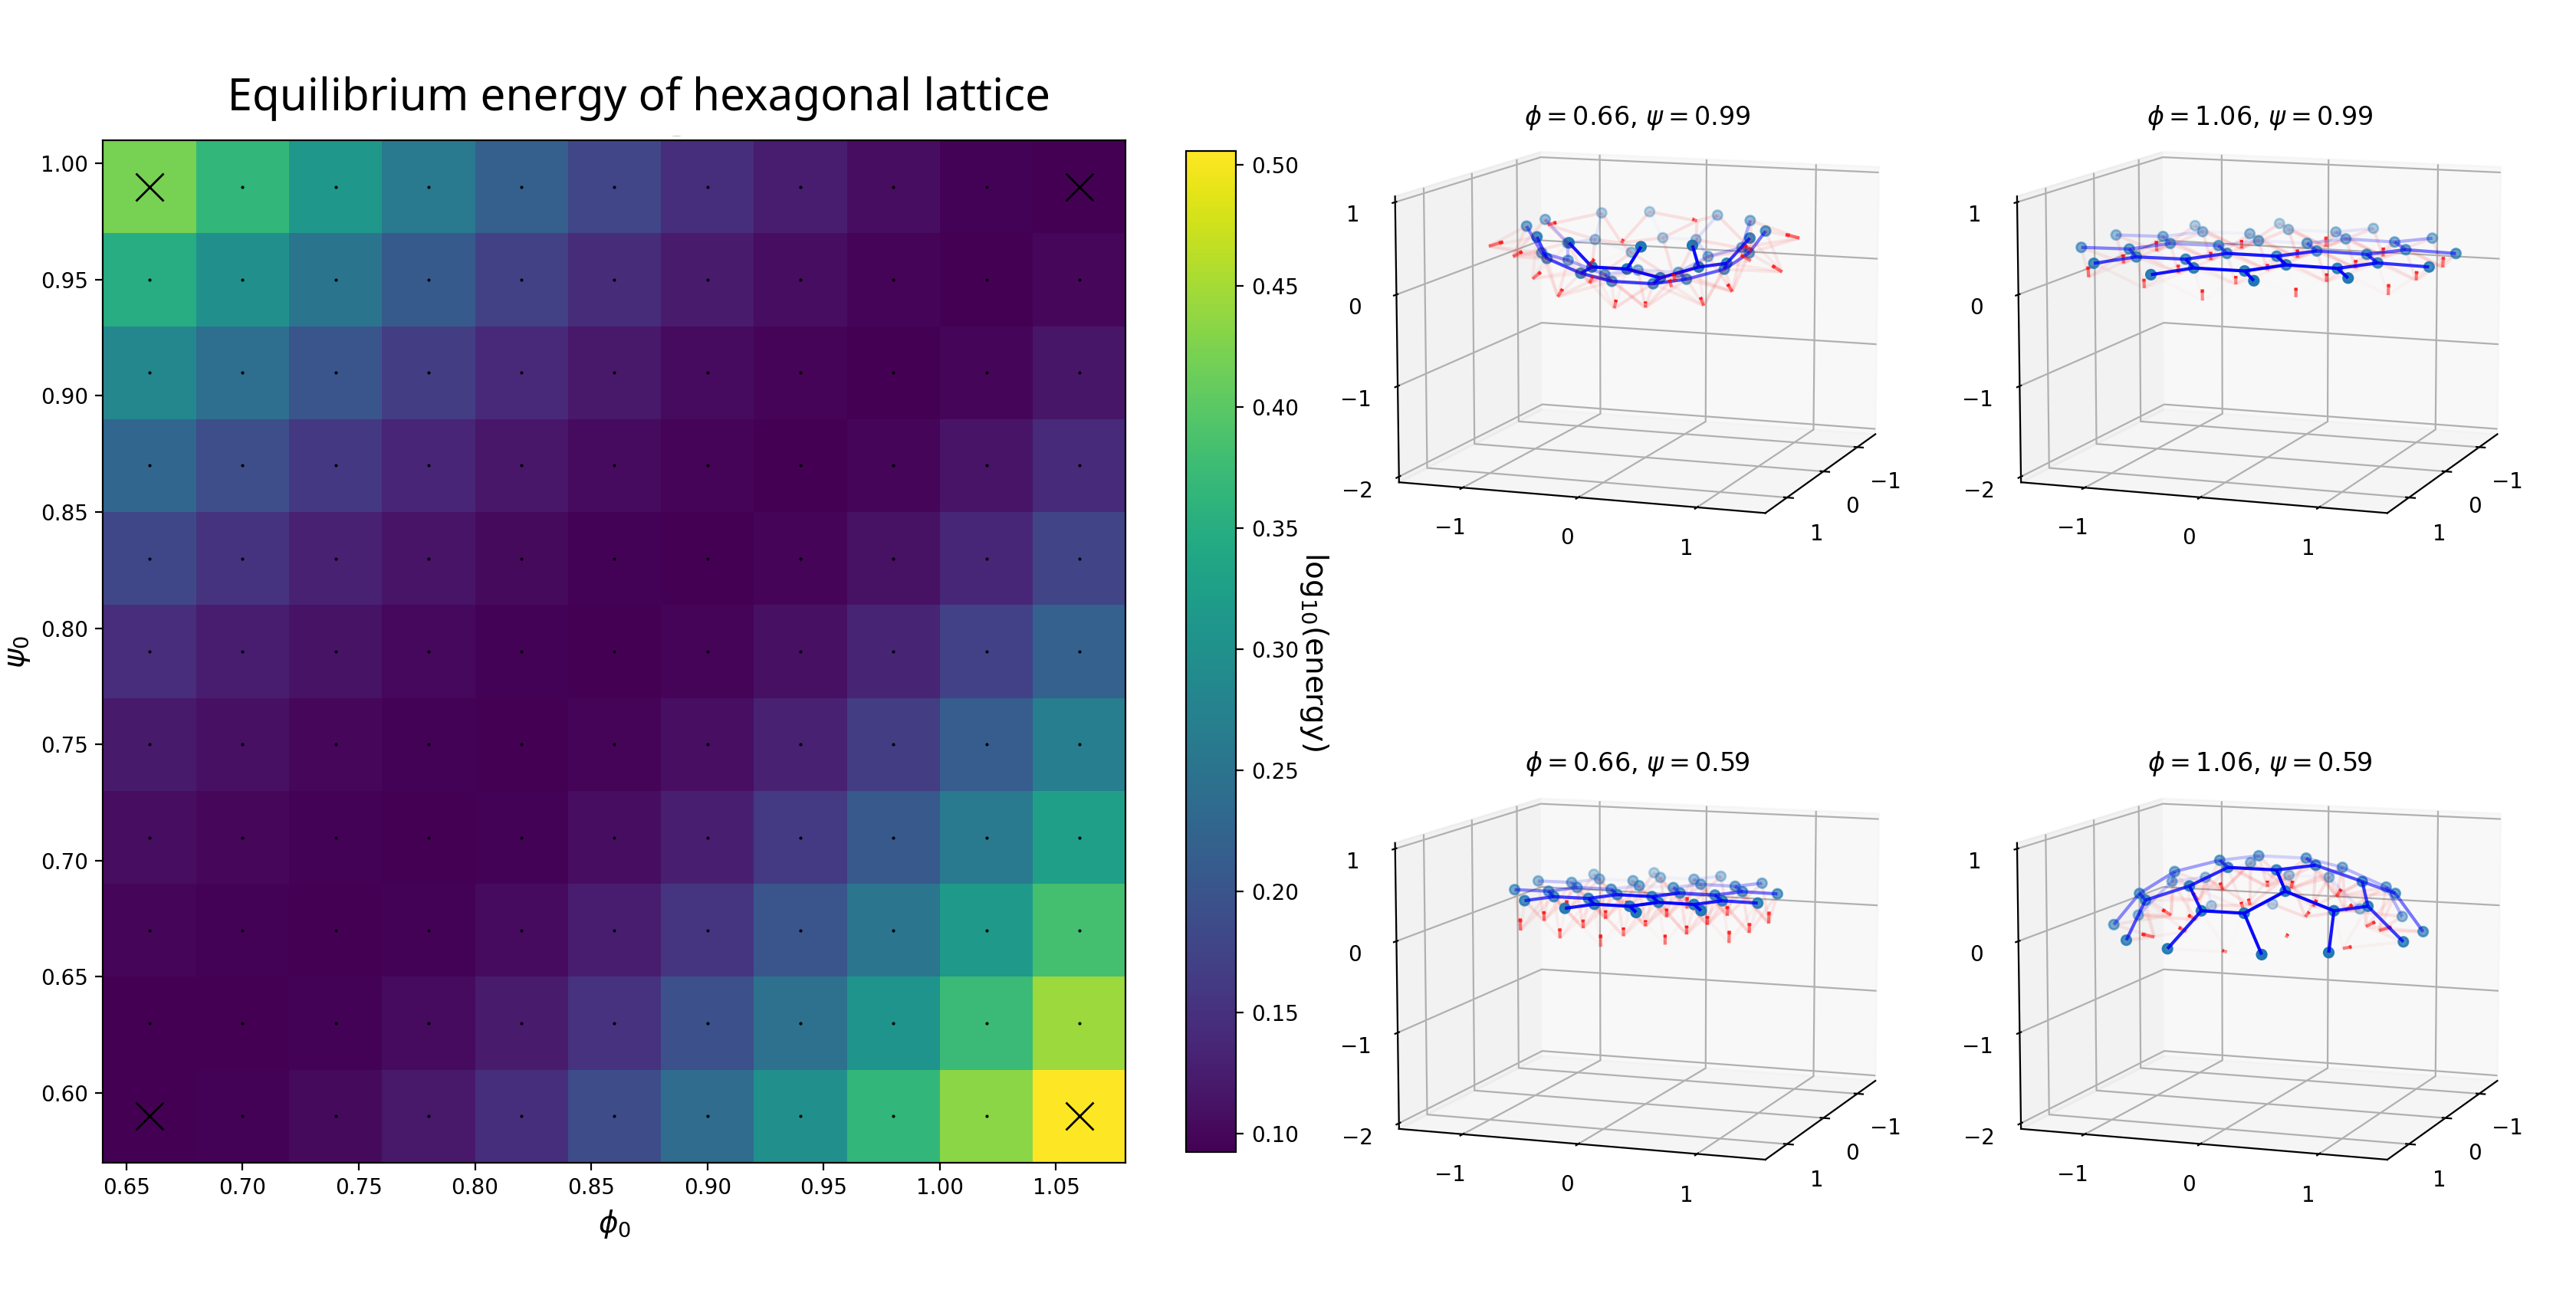
\includegraphics[width=\textwidth]{landscape_hex.png}
	\caption[Energy landscape of a discrete \textit{C. flexa} sheet generated from a hexagonal lattice]{Energy landcsape of a discrete \textit{C. flexa} sheet generated from a hexagonal lattice. Sheets displayed at the right correspond to the corners of the landscape indicated with white crosses. Energy along the diagonal is slightly above zero due to finite termination of gradient descent.}
	\label{fig:landscape_flat}
\end{figure}

We can observe a more rich energy landscape by using a graph topology containing defects from a hexagonal lattice.
A simple choice is an icosahedron, which is formed using a polyhedron of twelve vertices each of degree five forming twenty faces of equilateral triangles.
Each triangular face can each be repeatedly subdivided into four smaller equilateral triangular face by introducing a vertex along each edge, such that the surface gains vertices of degree six in a hexagonal lattice \citep{dahl2014}.
Intuitively, the fixed number of vertices with degree five make it possible for the vertices to form a closed surface.
For example, the patchwork of a football is formed by replacing each degree-five vertex of an icosahedron with a regular pentagon, and the polygons on the surface are able to form a regular pattern while forming an overall curved surface due to the diversity of shapes present.
The cells in \cref{fig:landscape_ico,fig:landscape_ico3,fig:landscape_ico4} sit at the vertices of icosahedra with two subdivisions, and the number of neighbours of each cell is visible by counting edges in the shapes defined by blue lines of the collar-collar interfaces.
Since cells with five neighbours form pentagons at their interfaces with other cells and cells with six neighbours form hexagons, the graph of collar-collar interactions matches that of a football.

A flexa sheet with collar-collar boundaries defined along a small section of the icosphere gives an energy landscape with two diagonal valleys corresponding to flagella-in and flagella-out sheets (upper and lower, respectively) in \cref{fig:landscape_ico}.
That there are two valleys, rather than the one valley along $\phi_0 = \psi_0$, is interpreted to be the result of topological defects in the lattice structure that are essential to the construction of the icosphere. 
The two energy valleys achieve similar values for the minimum sheet energy, suggesting there is not necessarily any energetic preference to either state in this model.
The positive and negative sheet curvatures respectively, in the convention of \cref{ch:2} is consistent with how we expect $\phi_0$ and $\psi_0$ to induce spontaneous curvature (\cref{eq:h0}).
The continuity between the two valleys indicates that sheets are stably able to flatten and the minimum energy structures continuously transition between flagella-in and -out structures. 
The landscape was found to differ negligibly when an inverted sheet was used to initialise the simulations.

\begin{figure}[hbtp]
	\centering
	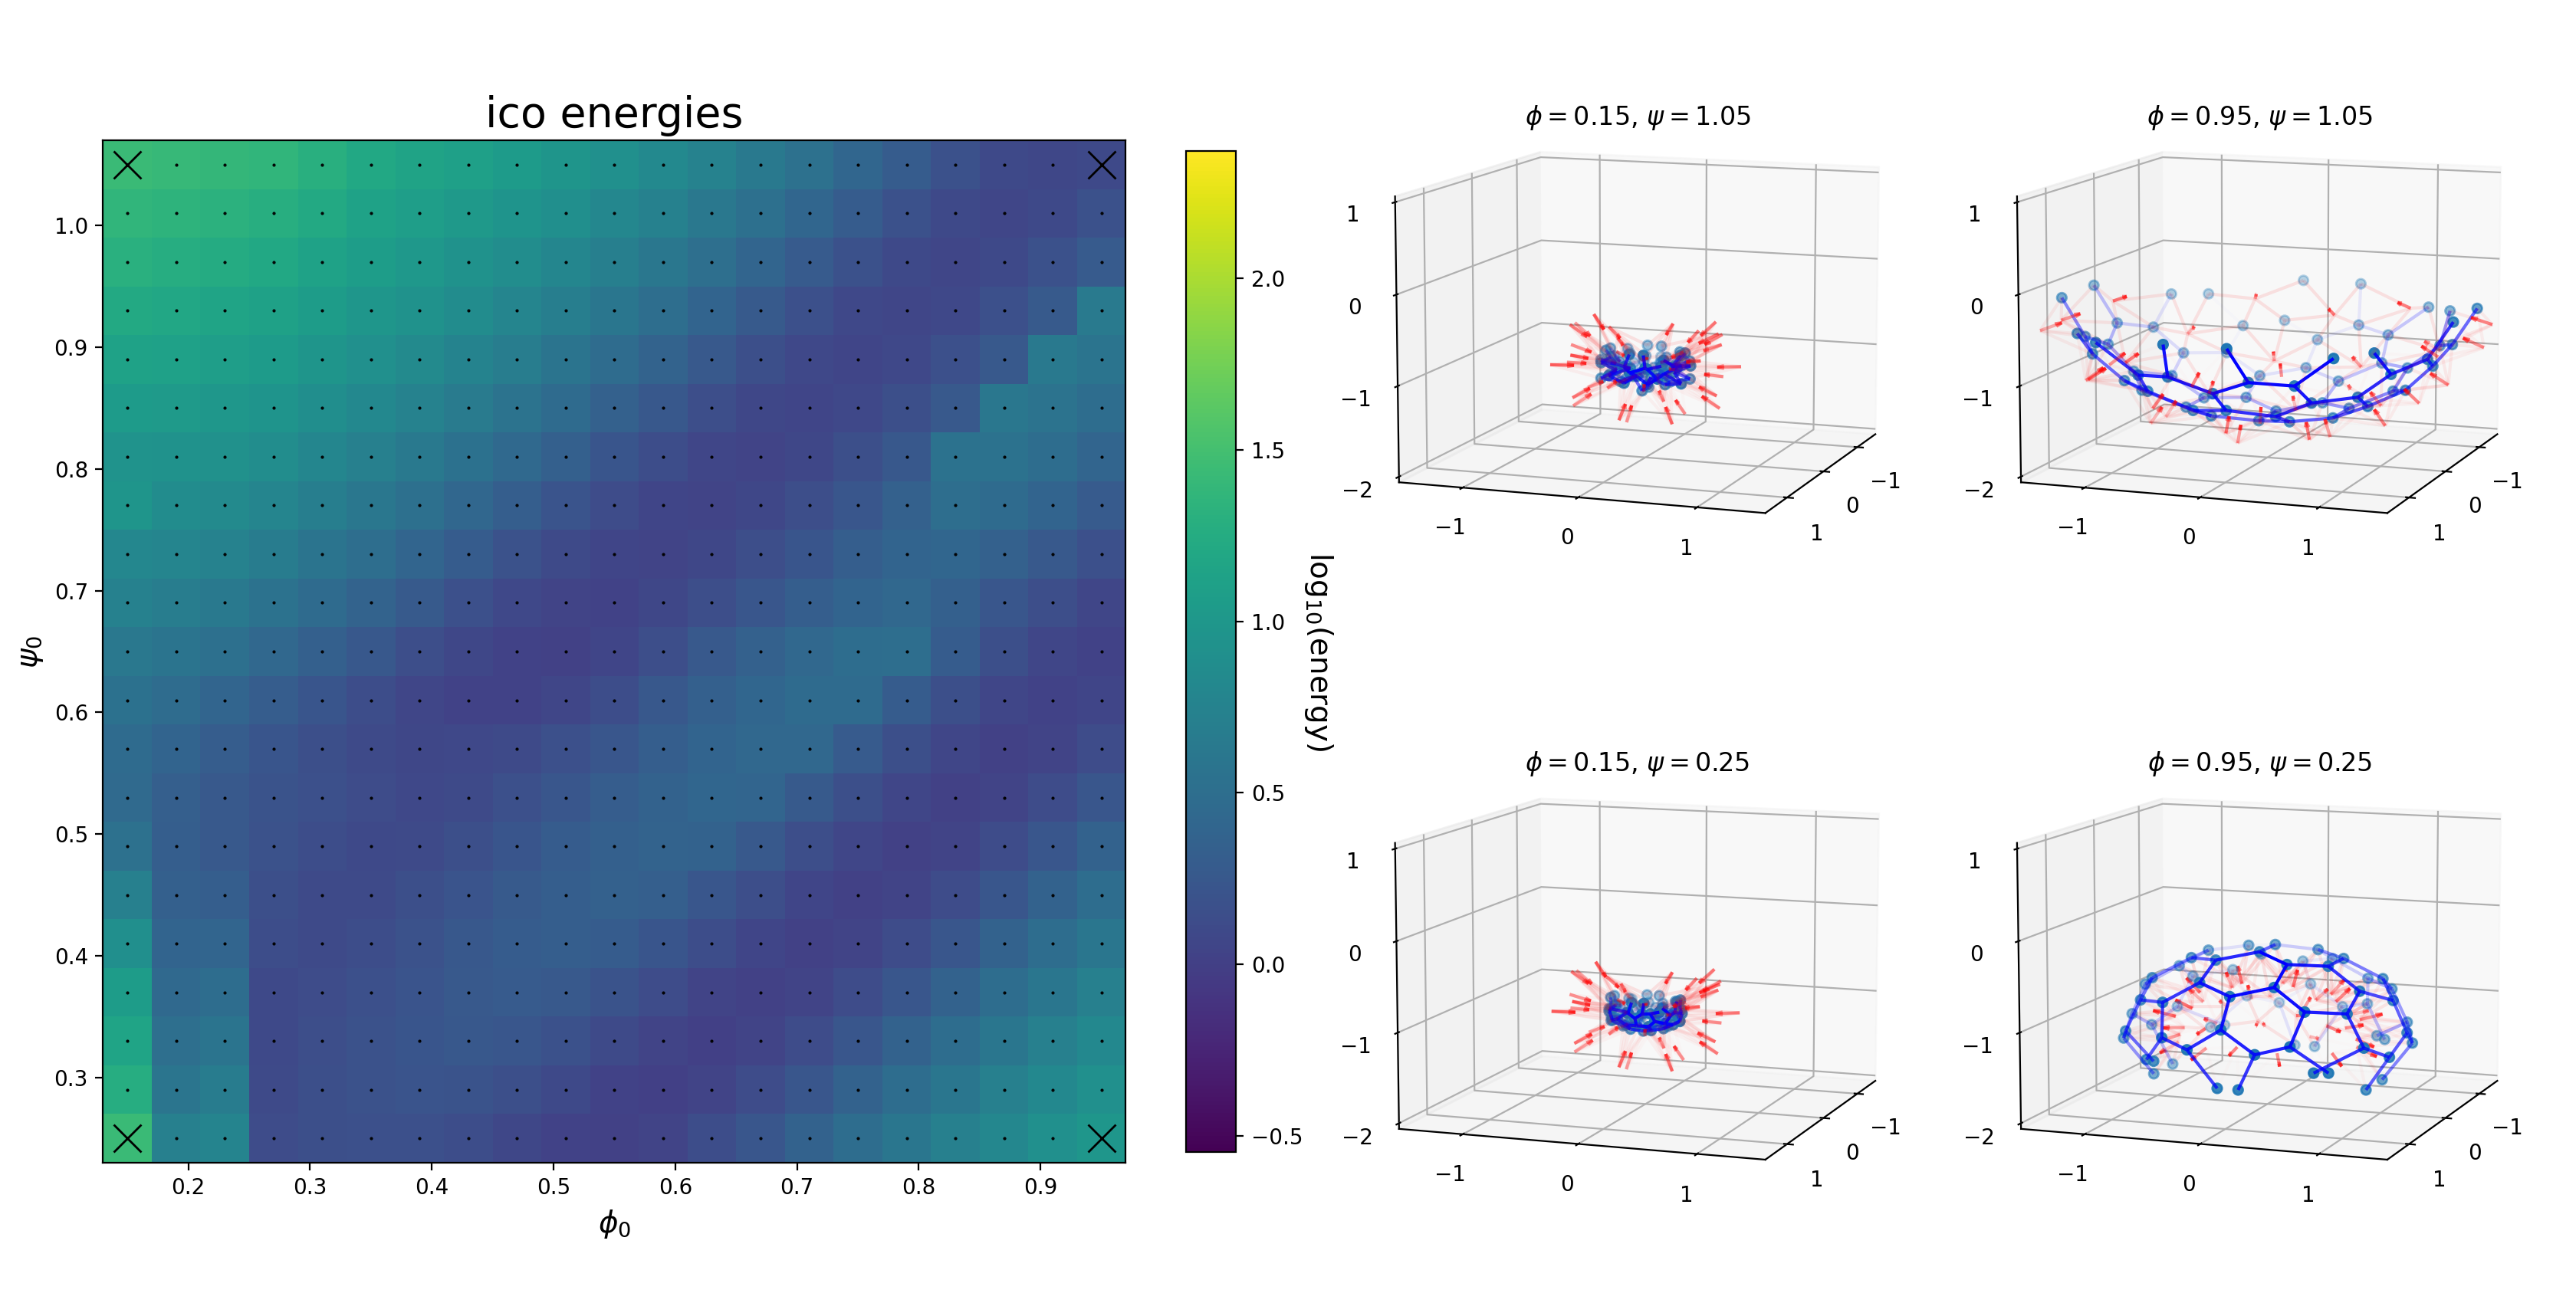
\includegraphics[width=\textwidth]{landscape_ico.png}
	\caption[Energy landscape of a discrete \textit{C. flexa} sheet generated from a small icosphere section]{Energy landscape of a discrete \textit{C. flexa} sheet generated from a thrice-subdivided icosphere section. Style as in \cref{fig:landscape_flat}. The icosphere was generated using code from \citep{dahl2014}. Cells comprising topological defects (those with five neighbours instead of the typical six) can be seen in the bottom-right-most panel, at the top right of the sheet and at the top left. The latter is difficult to see because the cell-cell collar interface boundaries (translucent blue points) are nearly collinear in the projection used to plot the sheet.}
	\label{fig:landscape_ico}
\end{figure}

\subsection{Sudden inversion}

Adding more cells by taking more vertices from the icosphere (with polar angle at least $2\pi/5$) again produces two energy valleys corresponding to flagella-in and -out sheets (\cref{fig:landscape_ico3}). 
In a larger sheet, however, we identify a discontinuity when beginning from a flagella-in sheet and changing parameters to achieve inversion (\cref{subfig:landscape_ico3}) as in \cref{fig:dynamics}.
The discontinuity implies that equilibrated sheets flagella-in sheets there achieve a local energy minimum, but that a global minimum may be achieved instead by taking a flagella-out sheet with the same parameters. 
Indeed, when using flagella-out sheets as initial conditions, the complete flagella-out energy valley is apparent and the discontinuity shifts to show the flagella-out to -in transition (\cref{subfig:landscape_ico3r}).\footnote{The large vertical discontinuity along $\phi_0=0.41$ is a consequence of the simulation parallelisation. All landscape plots shown were simulated by first equilibrating at the landscape centre ($\phi_0=0.55,\psi_0=0.65$). The row $\psi_0=0.65$ was simulated by using this as an initial condition to consecutively equilibrate to a larger or smaller value of $\phi_0$. Sheets were then simulated in columns from the central row for increasing or decreasing $\psi_0$. The vertical discontinuity indicates where the initial row simulations first transitioned, such that the sheets with $\phi_0=0.39$ in \cref{subfig:landscape_ico3r} began with a flagella-in sheet.}
Note that the sheet geometries at the landscape corners in \cref{fig:landscape_ico3} are the same, confirming inversion and the existence of unique minima in the landscape.

\begin{figure}
	\centering
	\begin{subfigure}[b]{\textwidth}
		\centering
		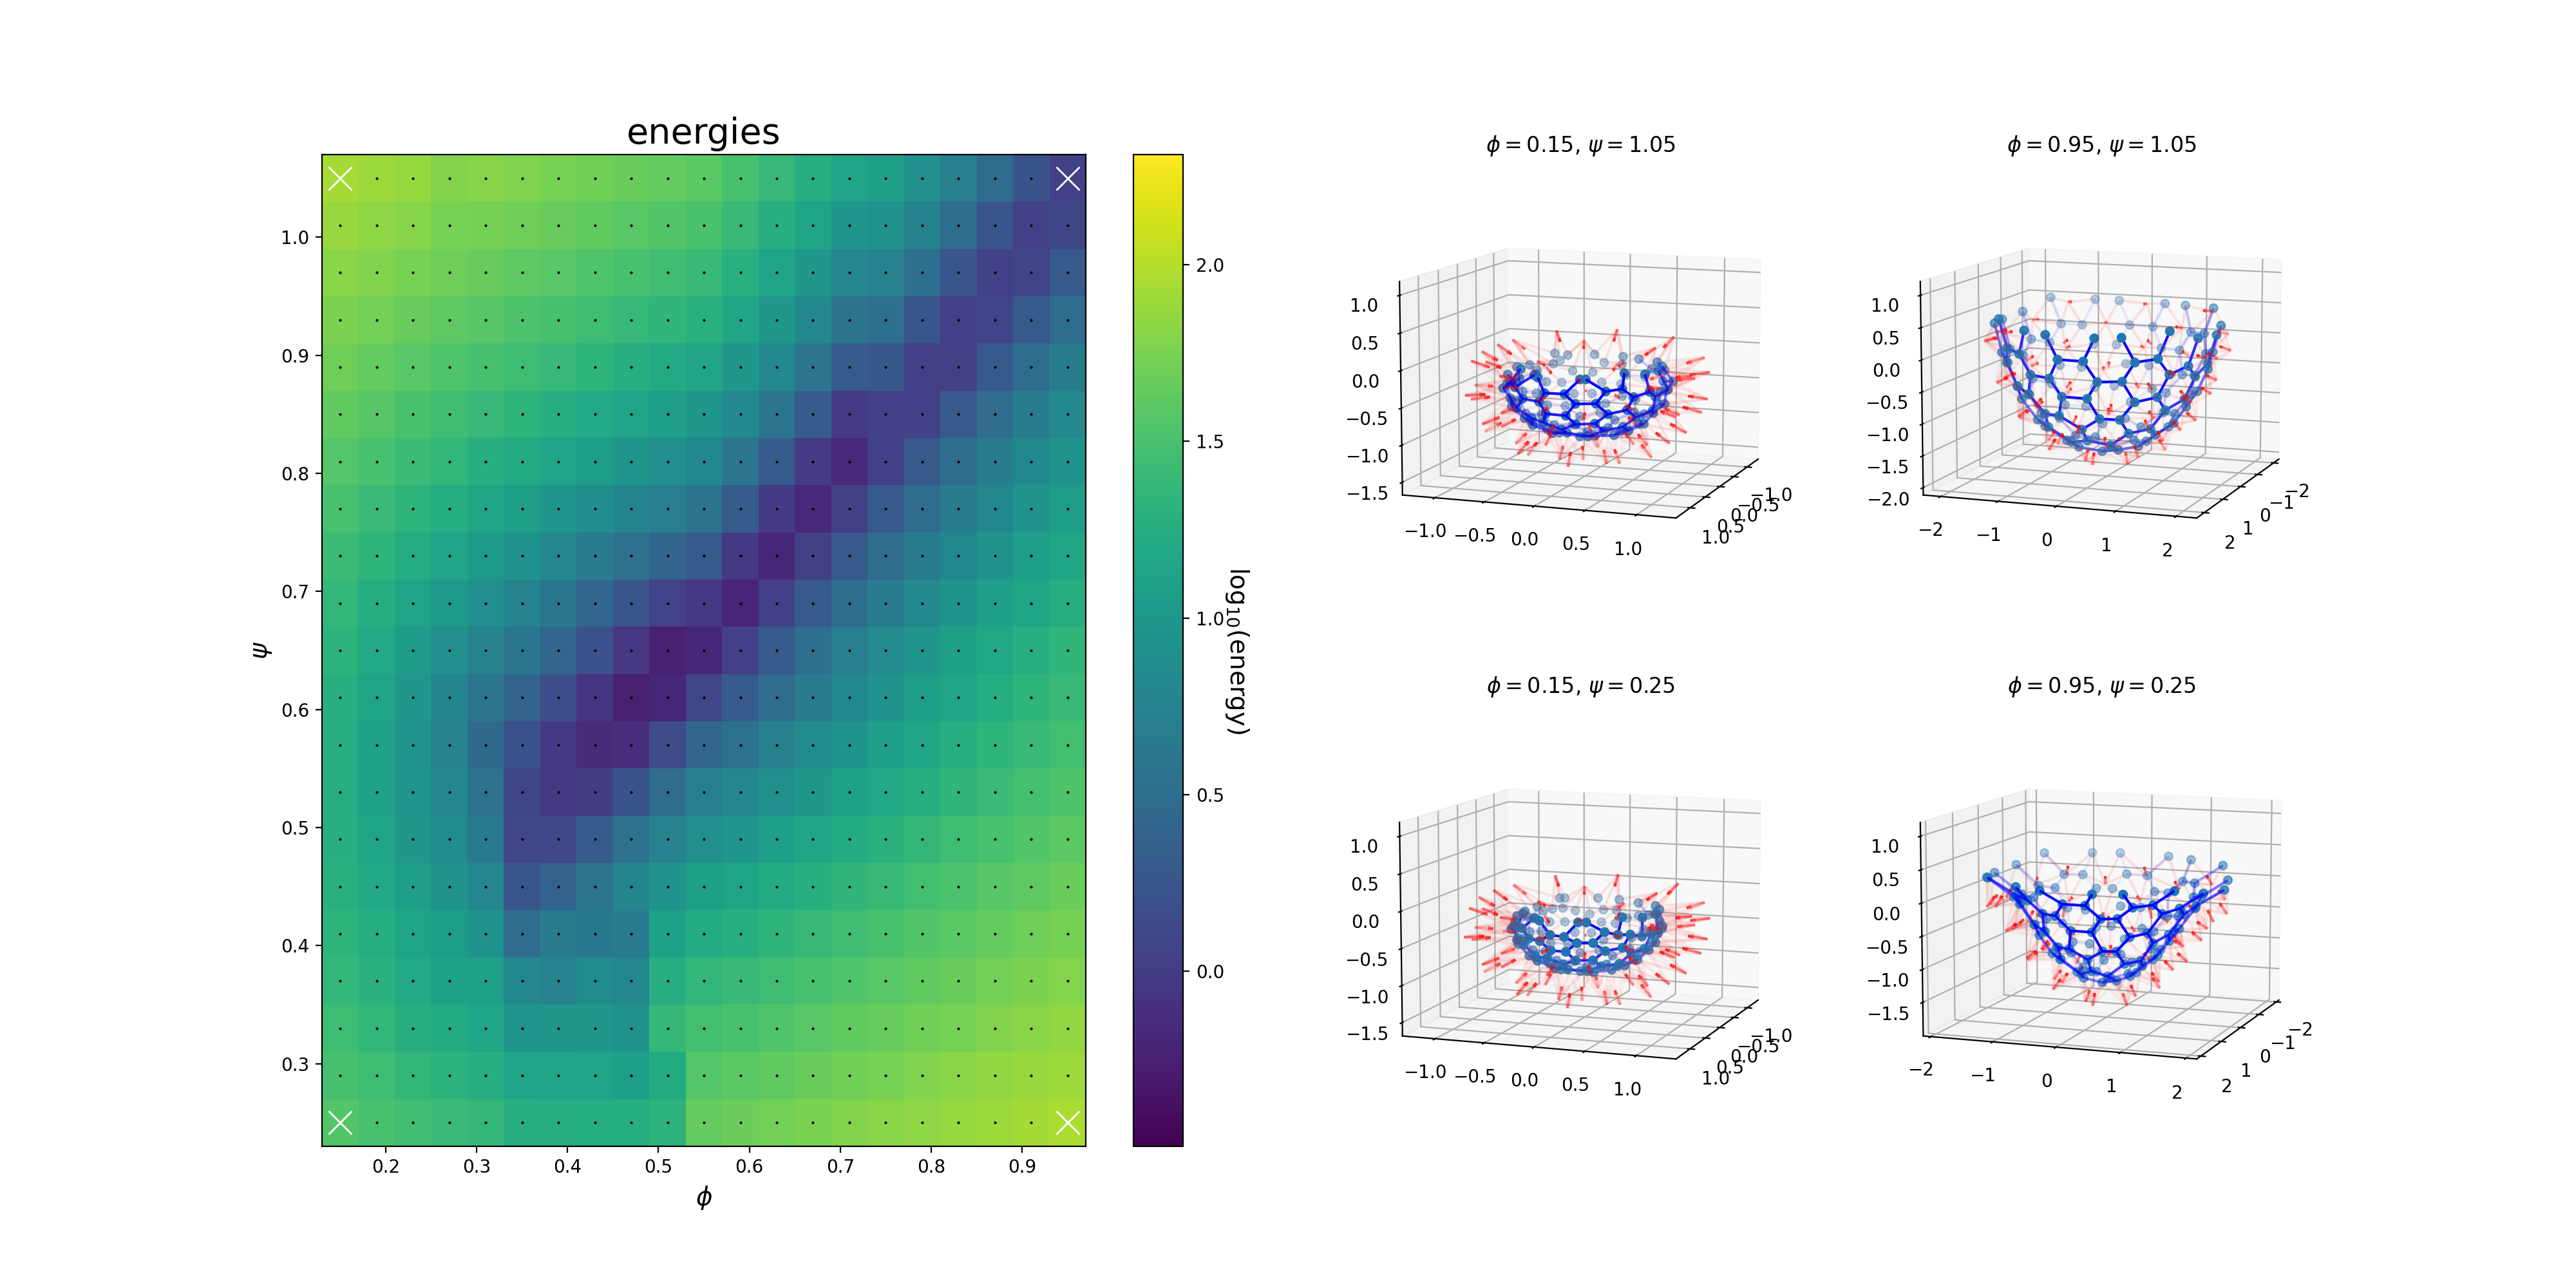
\includegraphics[width=\textwidth]{landscape_ico3.png}
		\caption{}
		\label{subfig:landscape_ico3}
	\end{subfigure}
	\begin{subfigure}[b]{\textwidth}
		\centering
		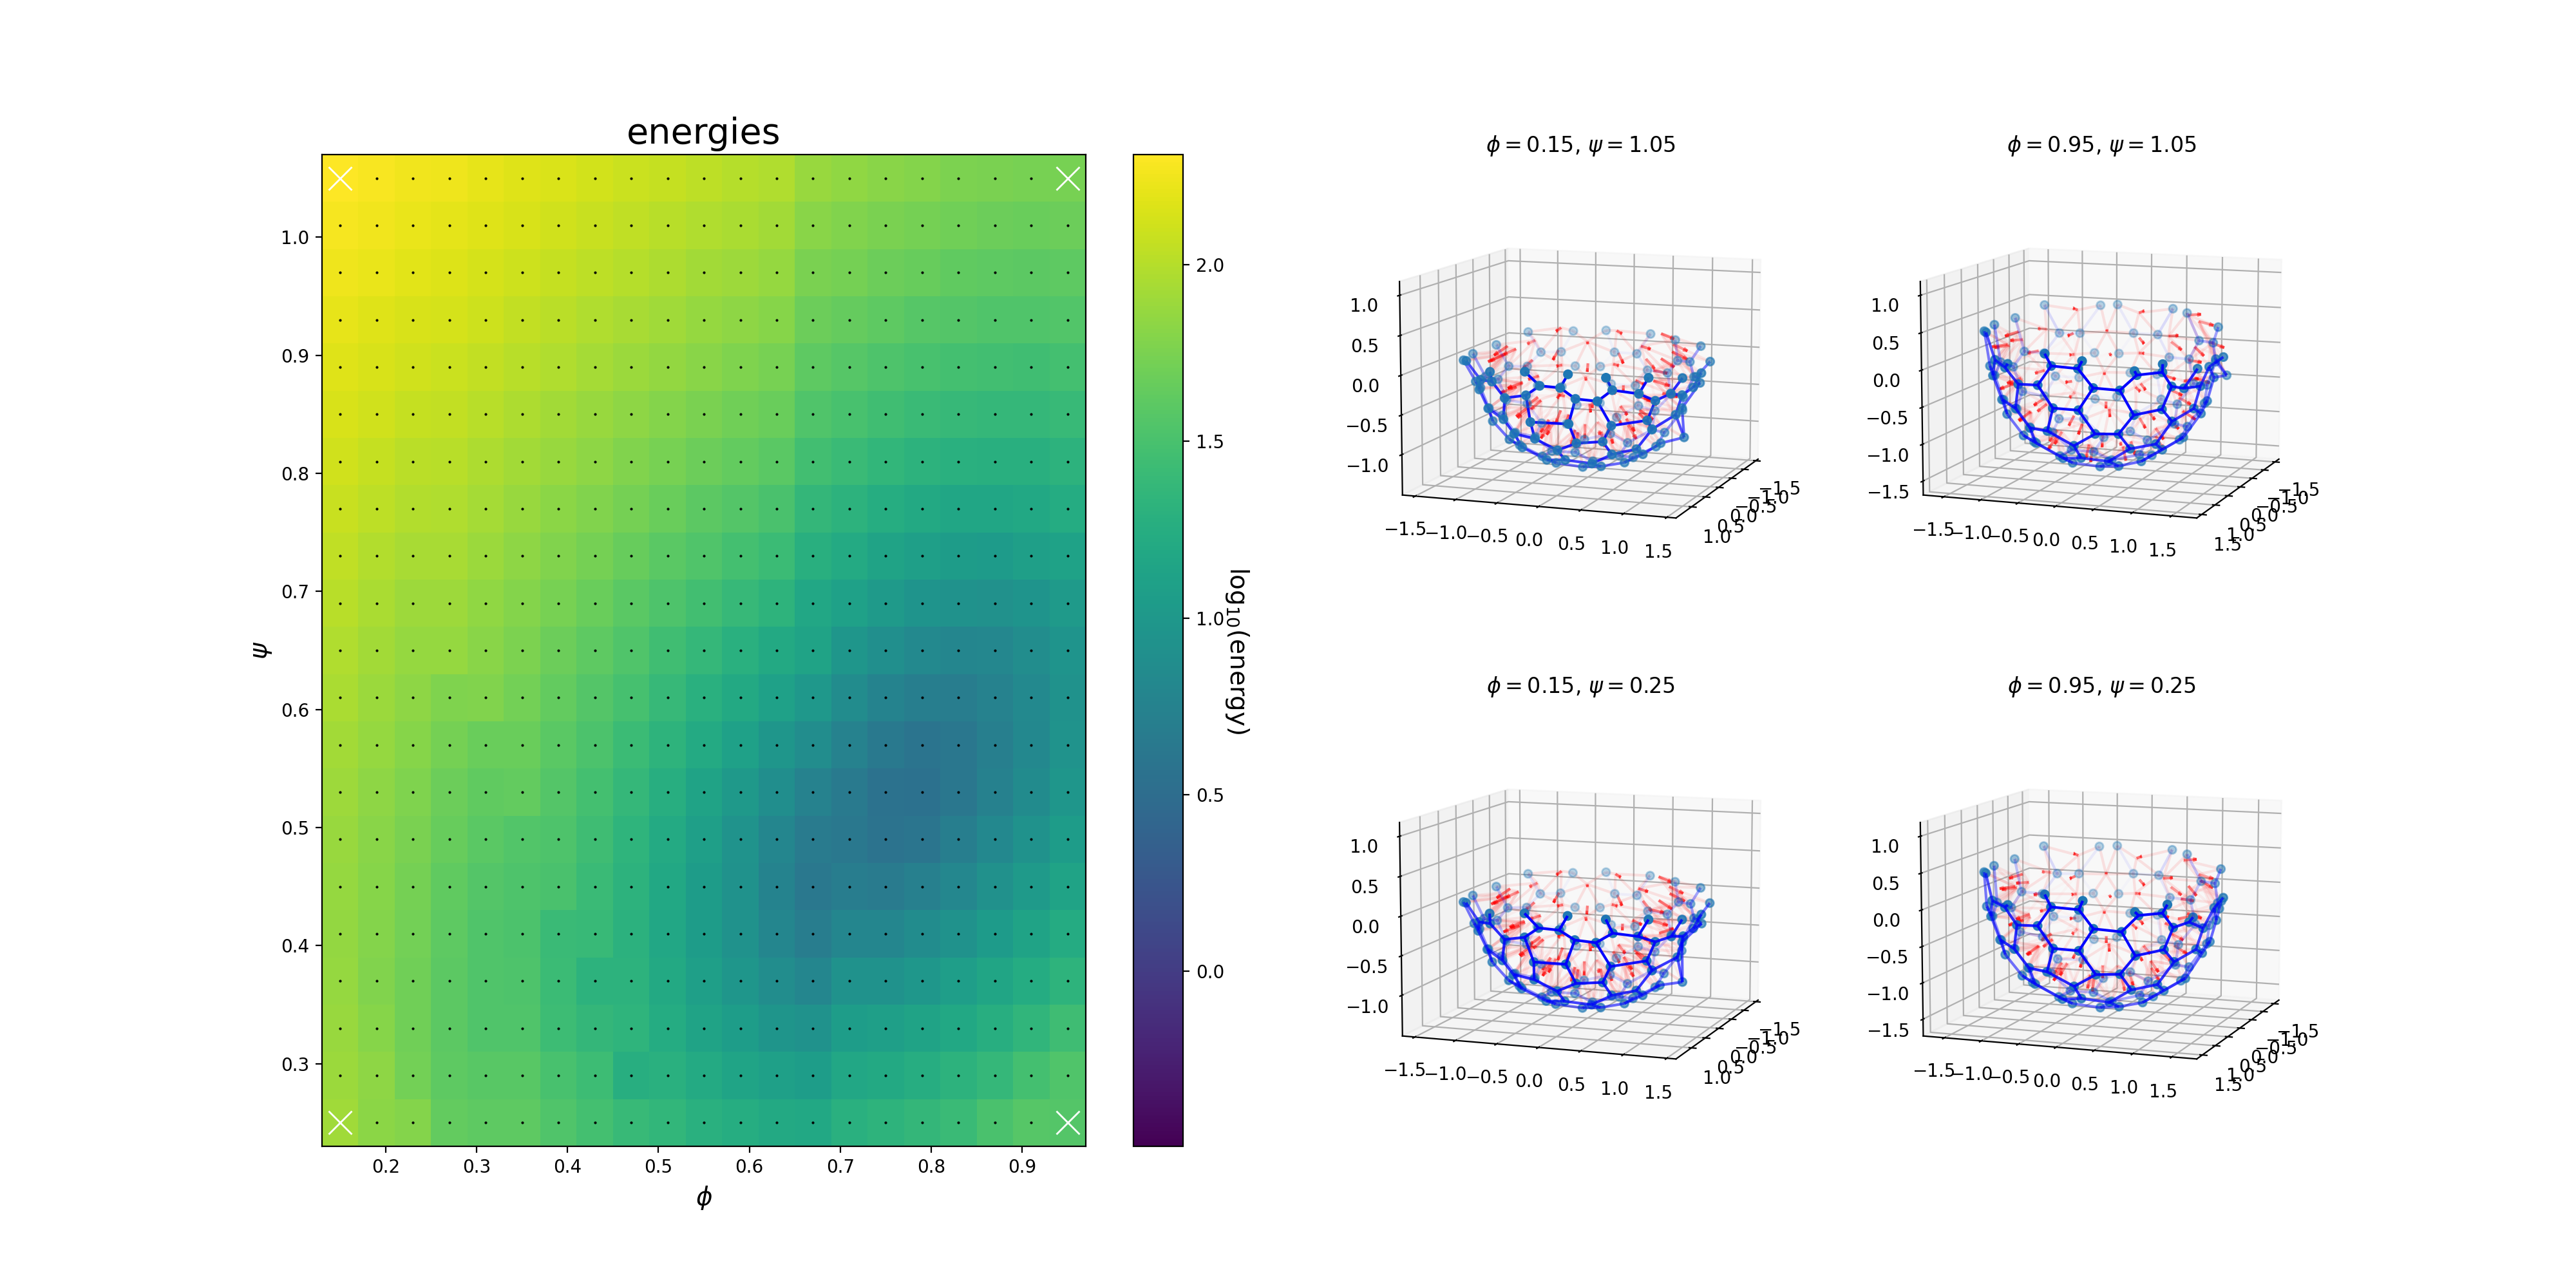
\includegraphics[width=\textwidth]{landscape_ico3r.png}
		\caption{}
		\label{subfig:landscape_ico3r}
	\end{subfigure}
	\caption[Energy landscape for flagella-in and flagella-out curved sheets]{Energy landscapes for (\ref{subfig:landscape_ico3}) flagella-in and (\ref{subfig:landscape_ico3r}) flagella-out sheets of \textit{C. flexa}. The color scaling is the same in both images. The landscapes for a smaller segment of the icosphere were qualitatively similar. Cells with five neighbours are easily visible in the bottom-right-most panel of \ref{subfig:landscape_ico3}, where one such cell is visible in the foreground and another is visible at the top right of the image.}
	\label{fig:landscape_ico3}
\end{figure}

As we are interested in the bistability and transition in \textit{C. flexa} sheets, we are concerned with the global energy minima for both flagella-in and -out sheets. 
In \cref{fig:landscape_merge}, the minimum energy geometries from the landscapes of \cref{fig:landscape_ico3} are shown with an indication which of the two plots the conformation came from.
The gloabl energy minima show two clear contiguous minimum energy valleys, as in \cref{fig:landscape_ico}.

\begin{figure}[ptbh]
	\centering
	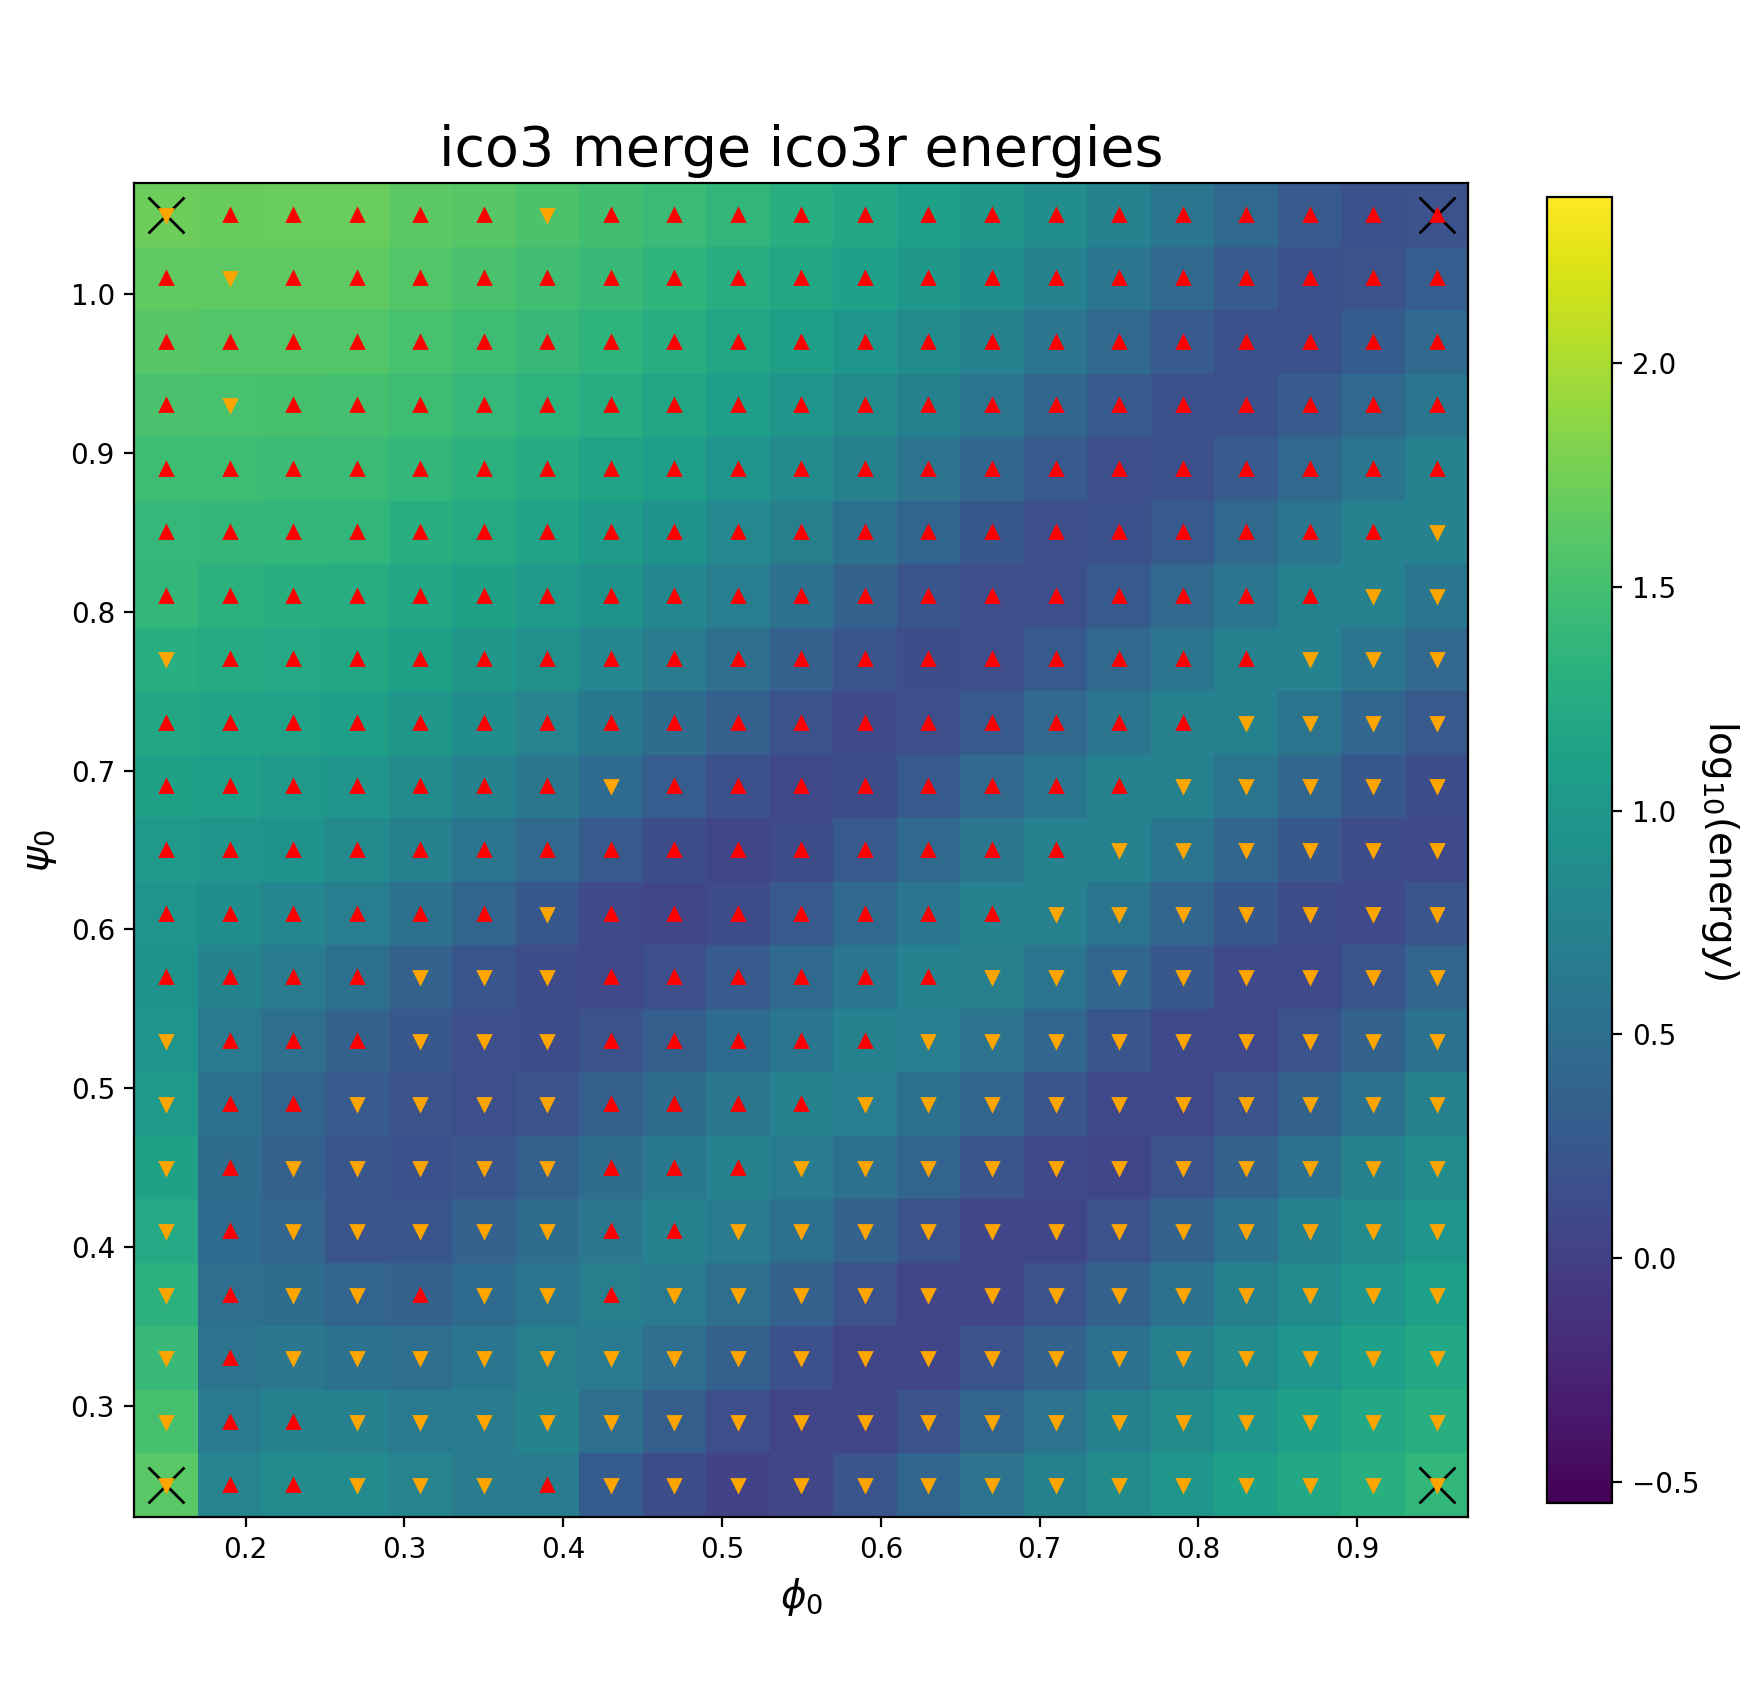
\includegraphics[width=\textwidth]{landscape_merge.png}
	\caption[Combined energy landscape of \cref{fig:landscape_ico3}]{Minimum energies the two landscapes shown in \cref{fig:landscape_ico3}. Values pulled from \cref{subfig:landscape_ico3} are denoted with red triangles and \cref{subfig:landscape_ico3r} with orange triangles.}
	\label{fig:landscape_merge}
\end{figure}

\Cref{eq:h0} describing the preferred mean curvature in terms of equilibrium constants $\phi_0$, $\psi_0$, and $\ell_0$ could be decomposed into a bending term $\sin(\psi_0 - \phi_0)$ and a length scale $\ell_0 \sin \phi_0$. 
Given the nearly constant behavior in \cref{fig:landscape_merge} along $\phi_0 = \psi_0$, it appears natural to project all points onto the orthogonal axis and plot the energy as a function of $\sin(\psi_0 - \phi_0)$. 
\Cref{fig:collapse} shows the result of plotting \cref{fig:landscape_merge} and the energies from \cref{fig:landscape_ico3} together. 
In this picture, we may interpret $\psi_0 - \phi_0$ as a state parameter to be varied causing a transition between flagella-in and -out states when sufficiently changed.

\begin{figure}[bthp]
	\centering
	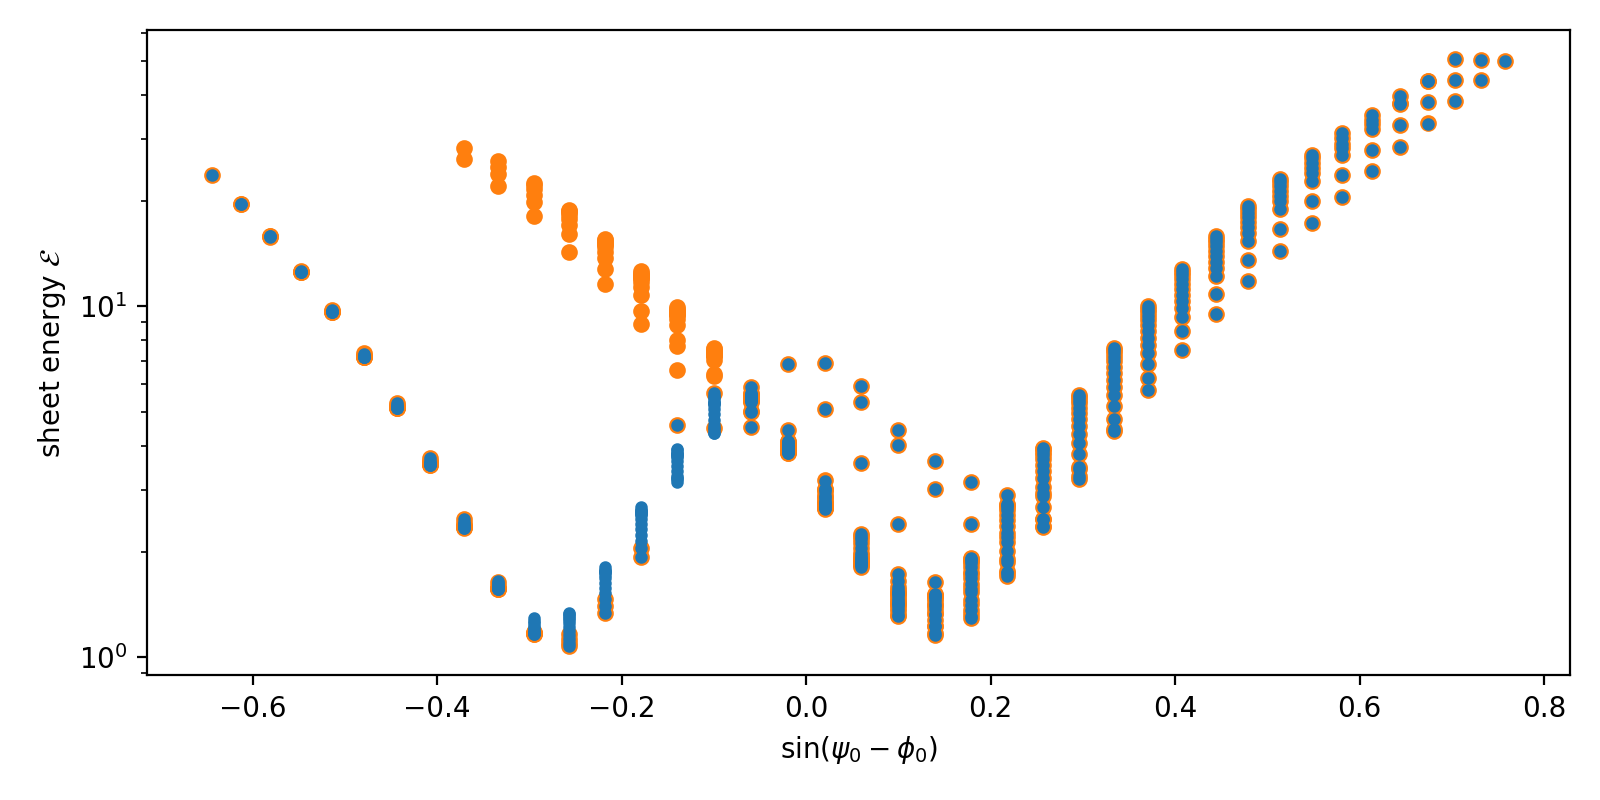
\includegraphics[width=\textwidth]{collapse.png}
	\caption[Energy landscape of an inverting sheet projected onto a single axis]{The energy landscapes in \cref{fig:landscape_merge} (blue points) and \cref{subfig:landscape_ico3} (orange, larger points) plotted as a function of $\sin (\psi_0 - \phi_0)$. Sheets beginning as flagella-in are able to exist in a stable local minimum that is not global.}
	\label{fig:collapse}
\end{figure}

\subsection{Inversion dynamics} \label{subsec:dynamics}

Informed by the transitions shown in the \cref{fig:landscape_ico3} landscape, we ask what the inversion dynamics look like in this model.
\Cref{fig:dynamics} shows the inversion from flagella-in to flagella-out by a single, sudden change in parameters.
Unlike the filament model studied in \cref{sec:c_1d} (\cref{fig:shapes}) and the small sheet in \cref{subsec:landscape}, large sheet inversion in the discrete model features temporary flattening through stretching at the edges.
The propagation of the change in curvature from the sheet boundary to the centre results in the \textit{rolling over} effect described in \cref{sec:c_1d} that is missing from those less detailed and smaller sheet descriptions. 
Notably, this is achieved with simple linear isotropic drag, supporting the hypothesis posed in \cref{sec:c_1d} that collar compression and stretching contribute meaningfully to inversion dynamics.

The continuities in \cref{fig:landscape_ico3} and inversion dynamics indicate that the topology of the cell-cell connection graph is key to producing bistability, where both flagella-in and flagella-out states are achievable as local energy minima for the same model parameters.
In contrast, a sheet without topological defects (\cref{fig:landscape_flat}) or a small sheet with fewer cells at the boundary (\cref{fig:landscape_ico}) readily inverts between states with similar energies.

Taking this further, we expect that some sheet topologies may be so restrictive at the boundary or elsewhere that inversion is completely prohibited for sufficiently high $k_{\text{sp}}$. 
Taking most of an icosphere to generate the sheet topology results in a complete inability to invert for the same energy constants used in \cref{fig:landscape_flat,fig:landscape_ico,fig:landscape_ico3}.
Instead, sheets retain their orientation always and experience substantial stress when the equilibrium angles prescribe a curvature that cannot be achieved in the present sheet orientation (\cref{fig:landscape_ico4}).
The flagella-out landscape is qualitatively similar with a valley in the same location as \cref{subfig:landscape_ico3r}.
The combined landscape of flagella-in and -out sheets (\cref{subfig:landscape4_merge}) again shows the two valleys, now separated by an insurmountable energetic barrier.

\begin{figure}
	\centering
	\begin{subfigure}[b]{\textwidth}
		\centering
		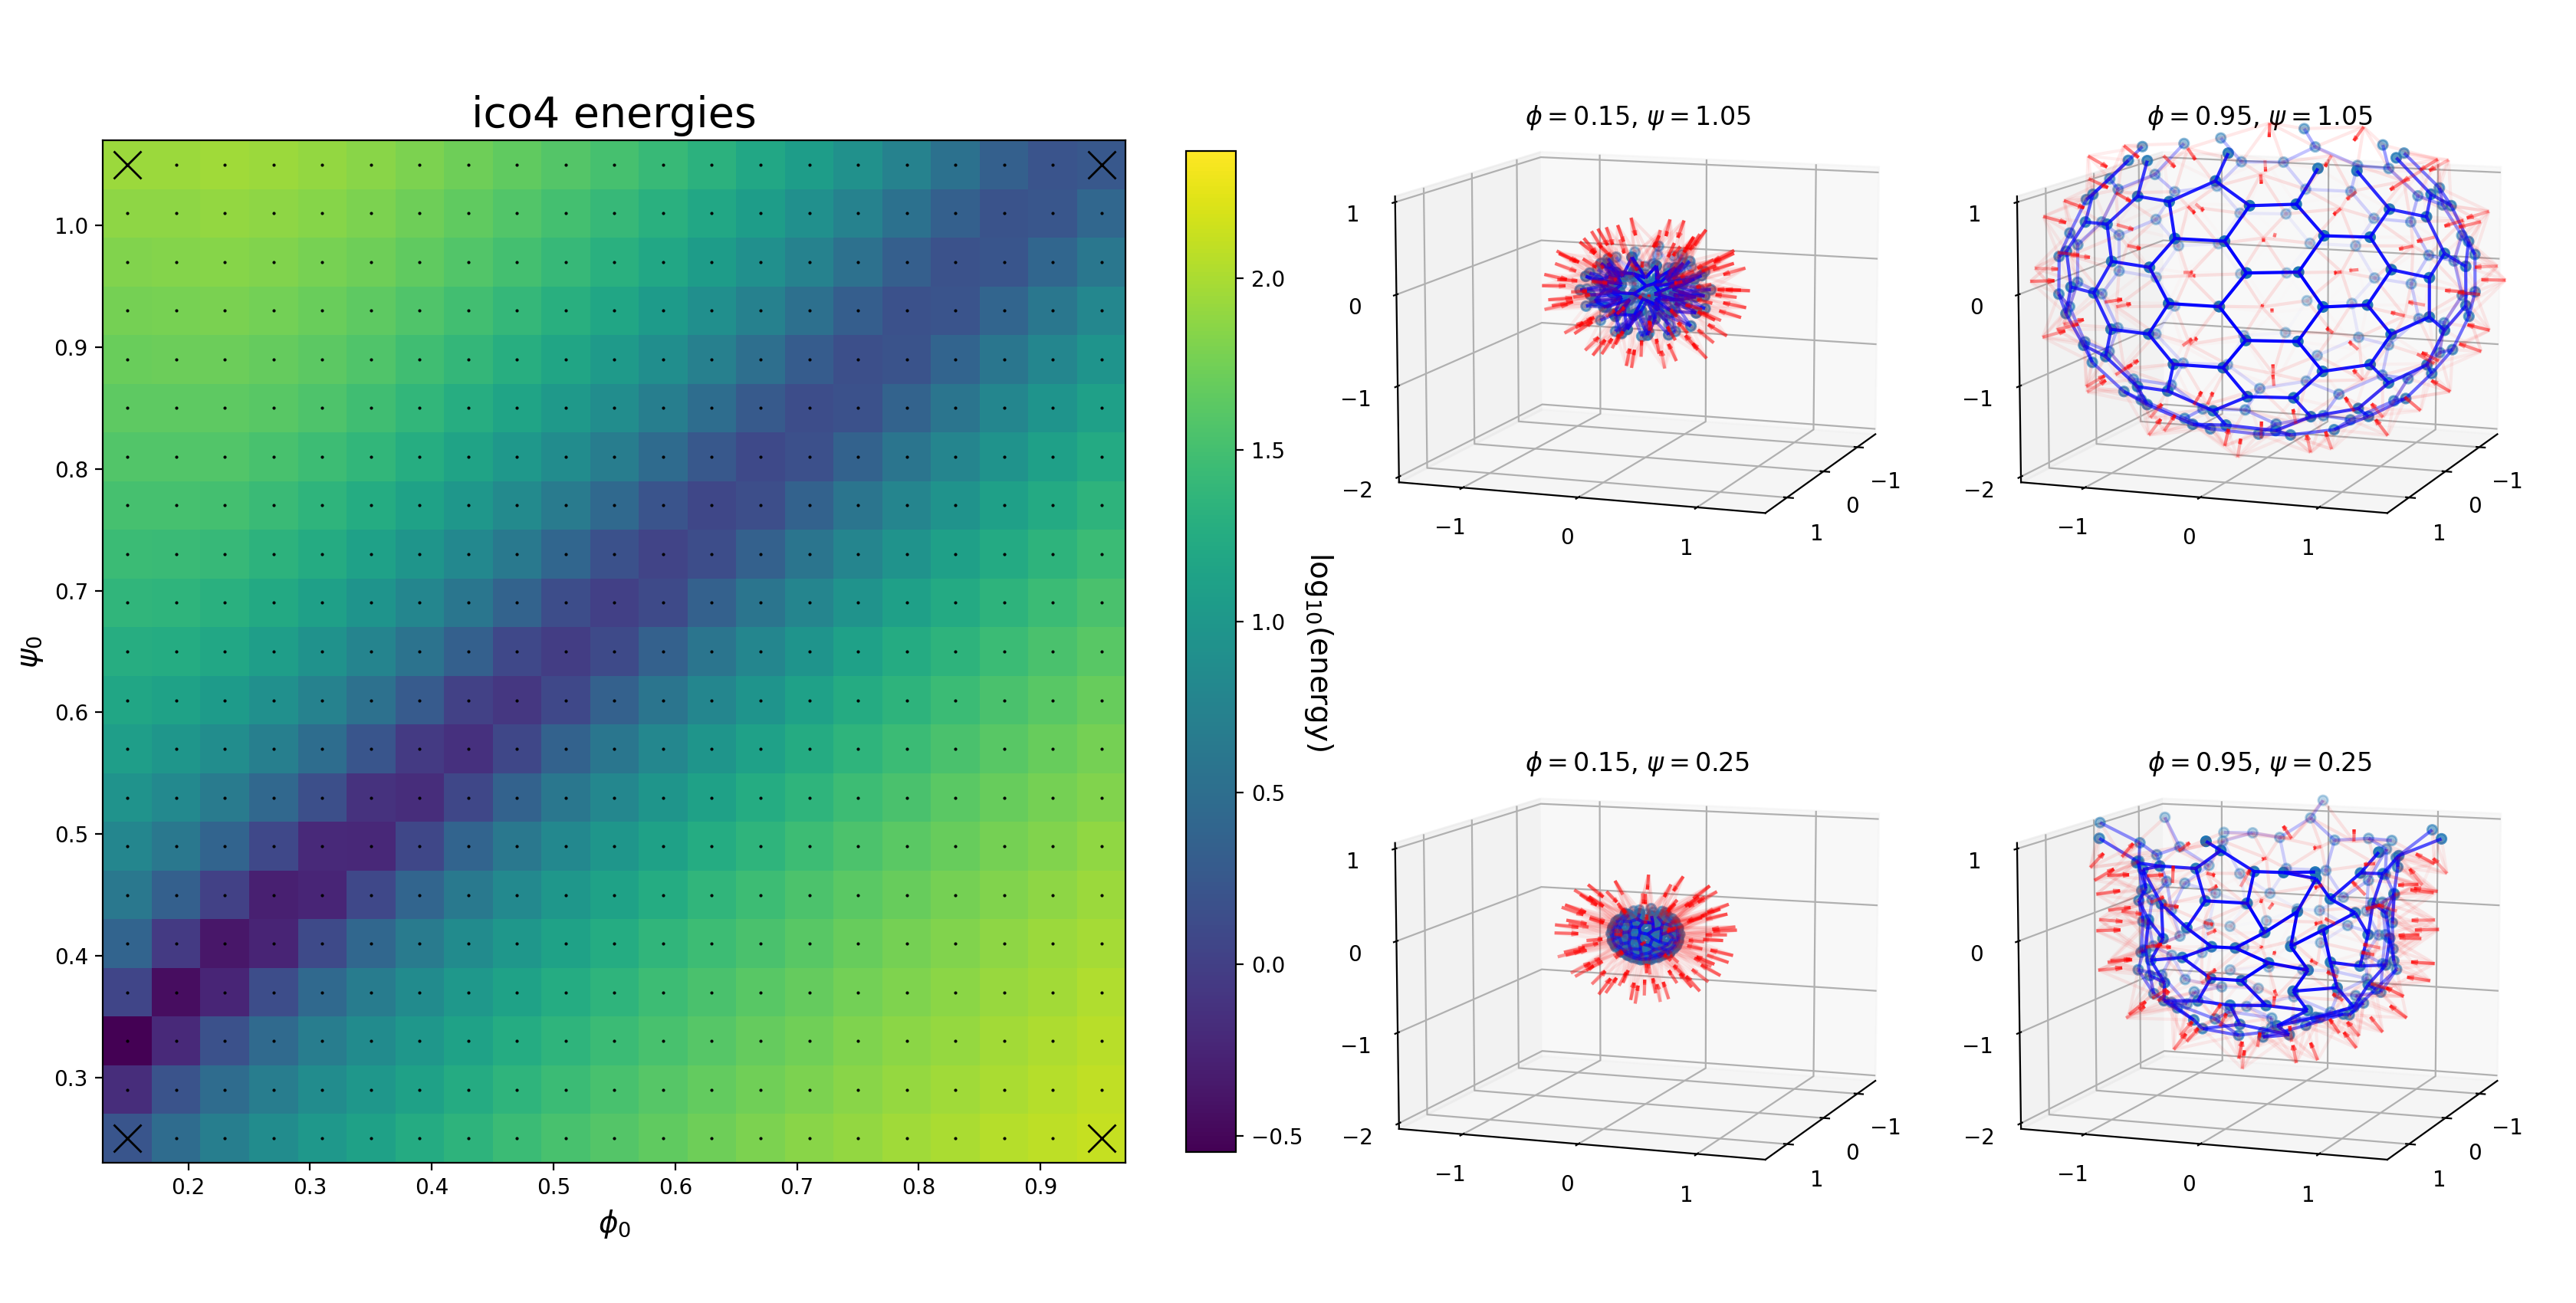
\includegraphics[width=\textwidth]{landscape_ico4.png}
		\caption{}
		\label{subfig:landscape_ico4}
	\end{subfigure}
	\begin{subfigure}[b]{\textwidth}
		\centering
		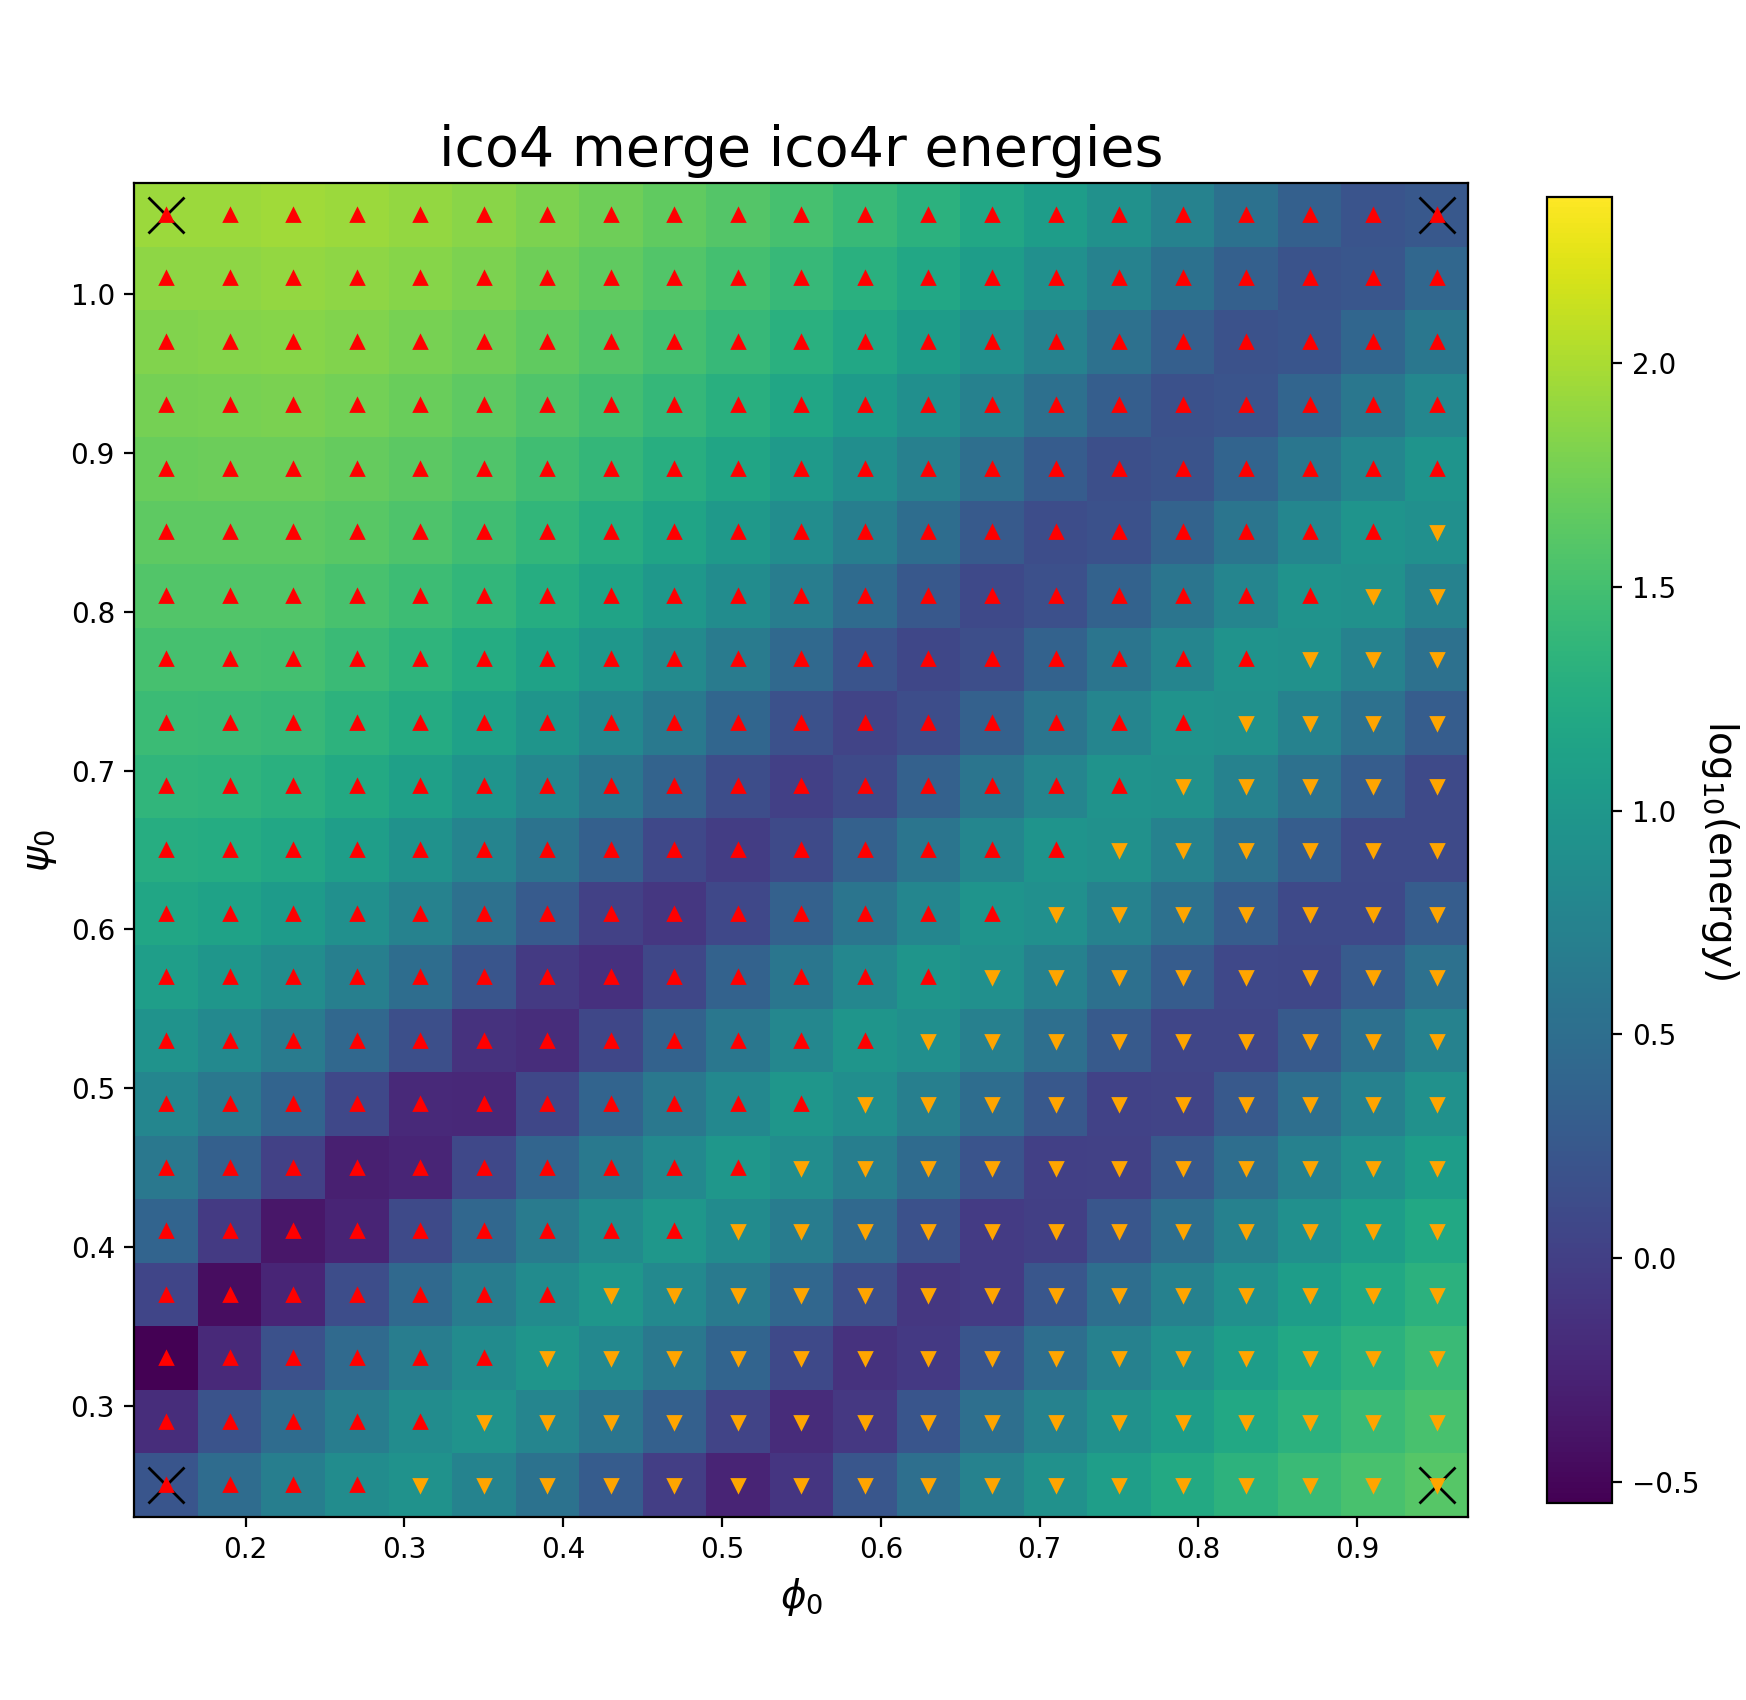
\includegraphics[width=0.8\textwidth]{landscape_ico4ico4r_merge.png}
		\caption{}
		\label{subfig:landscape4_merge}
	\end{subfigure}
	\caption[Energy landscape for flagella-in and flagella-out curved sheets]{(\ref{subfig:landscape_ico4}) Energy landscape for large flagella-in sheets. The landscape for flagella-out sheets was quantitatively similar, with the minimum energy valley shifted downward as in \cref{subfig:landscape_ico3r}. Several cells with an irregular number of neighbours are readily visible in the foreground of the top-left-most panel. (\ref{subfig:landscape4_merge}) Minimum energies for flagella-in and -out large sheets. Style as in \cref{fig:landscape_merge}.}
	\label{fig:landscape_ico4}
\end{figure}

It is clear that there may be a substantial energetic barrier to invert induced by collar-collar adhesion forces and collar stiffness. 
While this energetic barrier can be overcome by further pushing the equilibrium angles into a region that favors the opposite curvature (\cref{fig:landscape_ico3}) in simulations, \textit{C. flexa} cells appear to act in exclusively one of two pre-determined states.
There is no evidence to suggest changing collar properties, so we are led to predict that changing cell sheet topology is the factor which enables inversion.

\subsection{Additional graph topologies}

In addition to the hexagonal lattice and icosphere sections shown above, I observed that the lattice topology of the \textit{Choanoeca} sheet may restrict or force sheet bending altogether (\cref{fig:extra}).
A hexagonal lattice consisting of too many points is limited in its flexibility except at its edges (\cref{subfig:hexbig}). 
Consequently, we see that topological defects are not necessarily the hinderance to sheet bending or inversion, but rather necessary in moderation.
On the other hand, a sheet with many topological defects with topology formed by generalised Voronoi tesselation on the sphere using several random points is extremely restricted in curvature when there are too many points crowding a small region (\cref{subfig:sphere}).

\begin{figure}[bhtp]
	\centering
	\begin{subfigure}[b]{0.48\textwidth}
		\centering
		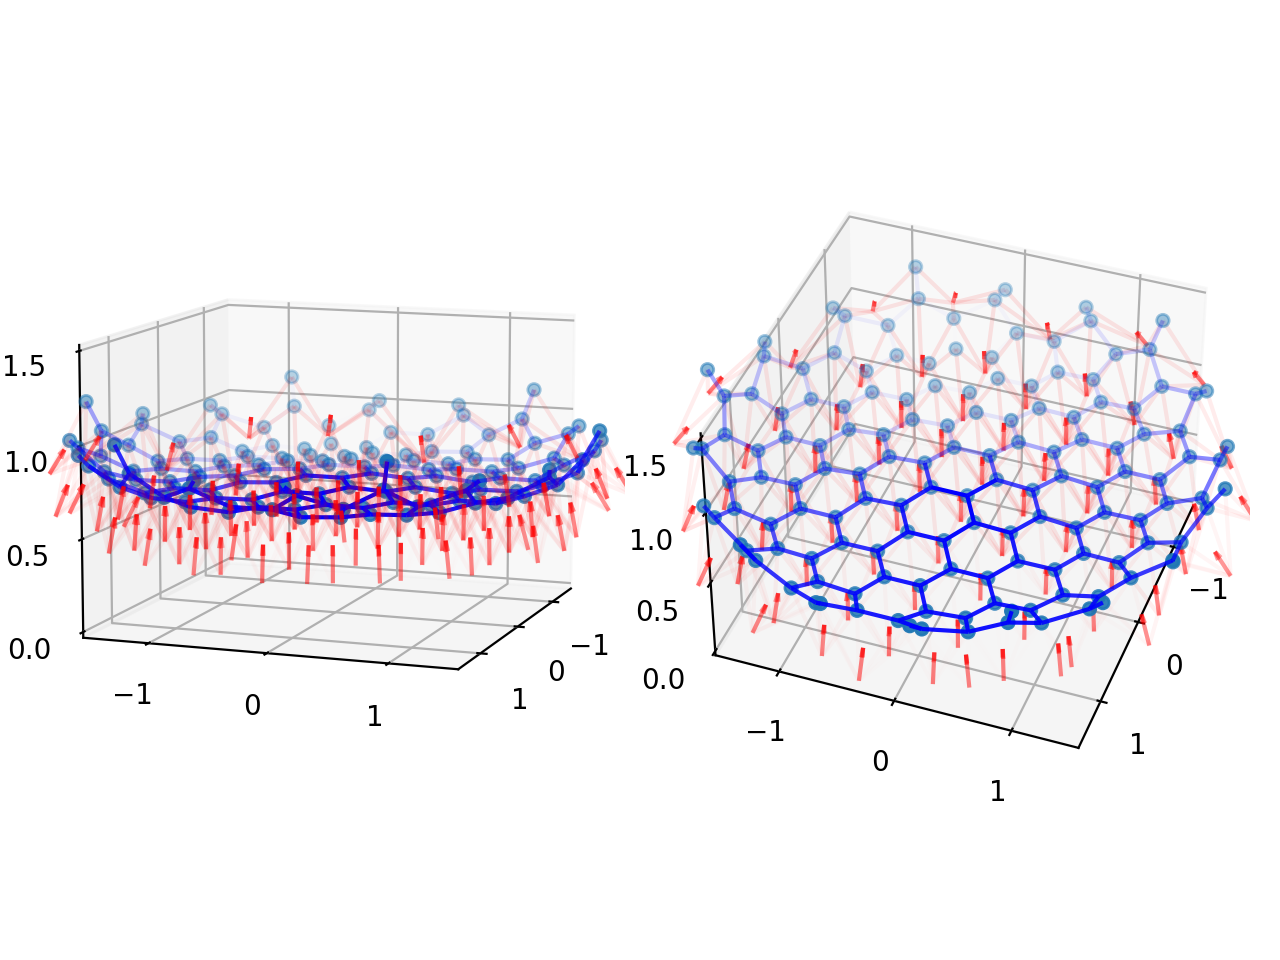
\includegraphics[width=\textwidth]{hexbig.png}
		\caption{}
		\label{subfig:hexbig}
	\end{subfigure}
	\begin{subfigure}[b]{0.48\textwidth}
		\centering
		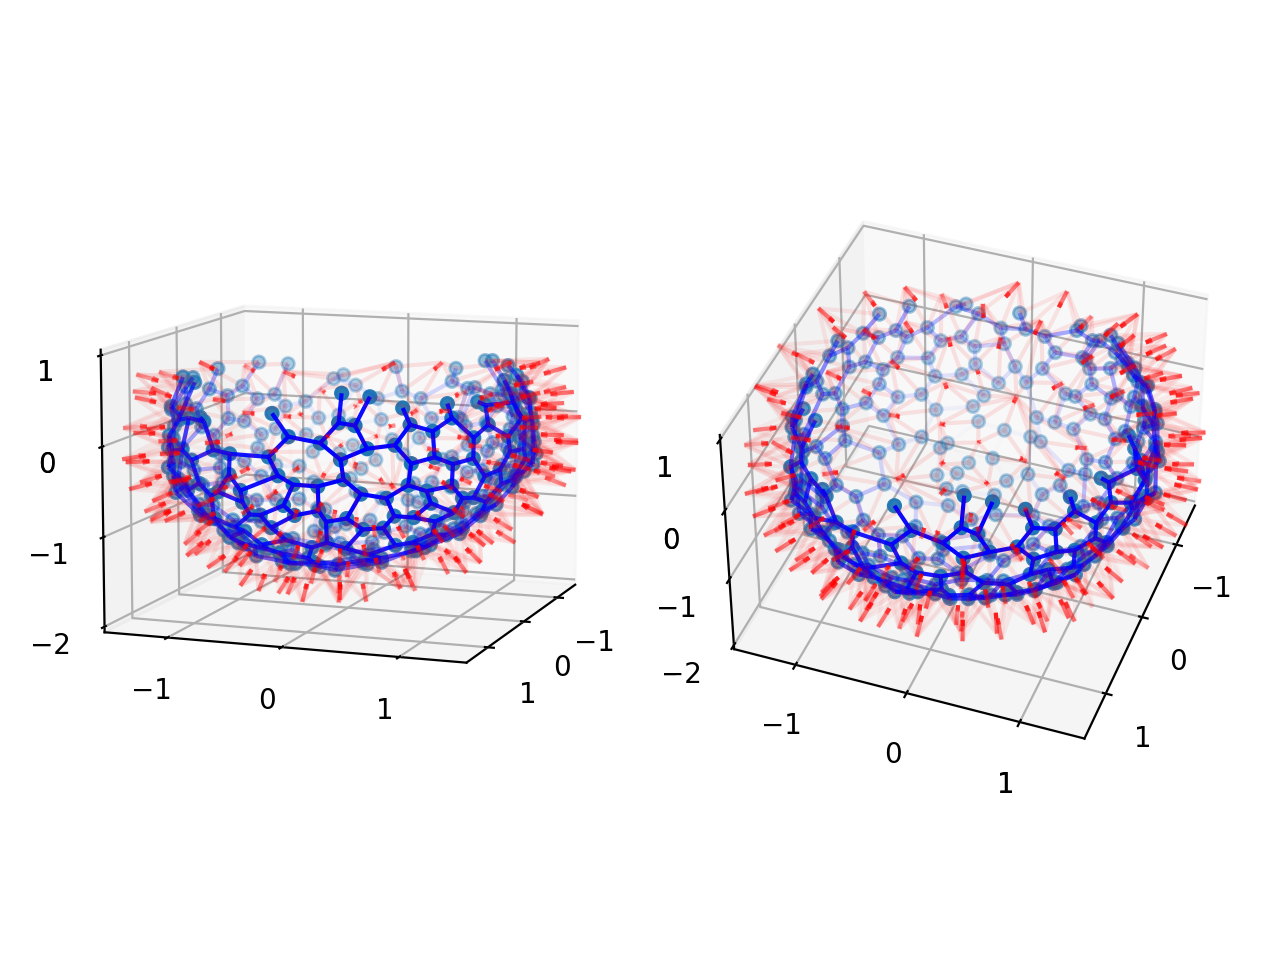
\includegraphics[width=\textwidth]{sphere.png}
		\caption{}
		\label{subfig:sphere}
	\end{subfigure}
	\caption[Equilibrium sheets of other lattice topologies]{Equilibrium sheets of additional lattice topologies. (\ref{subfig:hexbig}) Two views of a large hexagonal lattice sheet with $\phi_0 = 0.6$, $\psi_0 = 0.8$. Note that this angle caused substantial bending in \cref{fig:landscape_flat}. (\ref{subfig:sphere}) Two views of a sheet defined by Voronoi tesselation on random points on a sphere. The sheet was almost entirely rigid regardless of angles $\phi_0, \psi_0$ used.}
	\label{fig:extra}
\end{figure}

\mynote{Discuss that the phi and psi energies are around an order of magnitude higher than the spring energy? awaiting results from relaxing $k_{\text{sp}}$. Maybe it's really that you can't get expansion in collars at the boundary without expansion at the center too}

\begin{comment}
\begin{align*}
    \vec{F}_\gamma = \frac{\partial E}{\partial \vec{r}_\gamma} &= 2 \sum_{(\alpha, \rho)} \left( \phi_{(\alpha,\rho)} - \phi_0 \right) \frac{\partial \phi_{(\alpha,\rho)}}{\partial \vec{r}_\gamma} + 2 \sum_{(\alpha, \beta: \sigma, \rho)} \left( \psi(\hat{\bm{n}}_{\sigma\alpha\rho}, \hat{\bm{n}}_{\sigma\beta\rho}) - \psi_0 \right) \frac{\partial \psi_{(\alpha, \beta: \sigma, \rho)}}{\partial \vec{r}_\gamma} \\
    \frac{\partial \phi_{(\alpha,\rho)}}{\partial r_{\gamma i}} &= \frac{-1}{\sqrt{1 - (\hat{\bm{n}}_\alpha \cdot \hat{(\alpha\rho)})^2}} \left(\frac{\partial \hat{\bm{n}}_{\alpha j}}{\partial r_{\gamma i}} \hat{(\alpha\rho)}_j + \frac{\partial \hat{(\alpha\rho)}_j}{\partial r_{\gamma i}} \hat{\bm{n}}_{\alpha j} \right) \\
    \frac{\partial \hat{(\alpha\rho)}_j}{\partial r_{\gamma i}} &= \frac{(\delta_{\gamma\rho} - \delta_{\gamma\alpha})}{|r_\rho - r_\alpha|} \left( \delta_{ij} + \hat{(\alpha\rho)}_i\hat{(\alpha\rho)}_j \right) \\
    \frac{\partial \hat{\bm{n}}_{\alpha j}}{\partial r_{\gamma i}} &= \frac{\mathbb{1}_{\gamma\in \text{collars}(\alpha)} - n\delta_{\gamma\alpha}}{\left| \sum_{(\alpha, \rho)} (r_\rho - r_\alpha) \right|} \left(\delta_{ij} - \hat{\bm{n}}_{\alpha i} \hat{\bm{n}}_{\alpha j} \right) \\
    \frac{\partial \psi_{(\alpha, \beta: \sigma, \rho)}}{\partial r_{\gamma i}} &= \frac{-1}{\sqrt{1 - (\hat{\bm{n}}_{\rho\alpha\sigma} \cdot \hat{\bm{n}}_{\rho\beta\sigma}})^2} \left(\frac{\partial \hat{\bm{n}}_{\rho\alpha\sigma j}}{\partial r_{\gamma i}} \hat{\bm{n}}_{\rho\beta\sigma j} + \frac{\partial \hat{\bm{n}}_{\rho\beta\sigma j}}{\partial r_{\gamma i}} \hat{\bm{n}}_{\rho\alpha\sigma j} \right) \\
    \frac{\partial \hat{\bm{n}}_{\rho\alpha\sigma j}}{\partial r_{\gamma i}} &= \text{too big see notes}
\end{align*}
\end{comment}
